\documentclass[11pt]{article}

    \usepackage[breakable]{tcolorbox}
    \usepackage{parskip} % Stop auto-indenting (to mimic markdown behaviour)
    
    \usepackage{iftex}
    \ifPDFTeX
    	\usepackage[T1]{fontenc}
    	\usepackage{mathpazo}
    \else
    	\usepackage{fontspec}
    \fi

    % Basic figure setup, for now with no caption control since it's done
    % automatically by Pandoc (which extracts ![](path) syntax from Markdown).
    \usepackage{graphicx}
    % Maintain compatibility with old templates. Remove in nbconvert 6.0
    \let\Oldincludegraphics\includegraphics
    % Ensure that by default, figures have no caption (until we provide a
    % proper Figure object with a Caption API and a way to capture that
    % in the conversion process - todo).
    \usepackage{caption}
    \DeclareCaptionFormat{nocaption}{}
    \captionsetup{format=nocaption,aboveskip=0pt,belowskip=0pt}

    \usepackage[Export]{adjustbox} % Used to constrain images to a maximum size
    \adjustboxset{max size={0.9\linewidth}{0.9\paperheight}}
    \usepackage{float}
    \floatplacement{figure}{H} % forces figures to be placed at the correct location
    \usepackage{xcolor} % Allow colors to be defined
    \usepackage{enumerate} % Needed for markdown enumerations to work
    \usepackage{geometry} % Used to adjust the document margins
    \usepackage{amsmath} % Equations
    \usepackage{amssymb} % Equations
    \usepackage{textcomp} % defines textquotesingle
    % Hack from http://tex.stackexchange.com/a/47451/13684:
    \AtBeginDocument{%
        \def\PYZsq{\textquotesingle}% Upright quotes in Pygmentized code
    }
    \usepackage{upquote} % Upright quotes for verbatim code
    \usepackage{eurosym} % defines \euro
    \usepackage[mathletters]{ucs} % Extended unicode (utf-8) support
    \usepackage{fancyvrb} % verbatim replacement that allows latex
    \usepackage{grffile} % extends the file name processing of package graphics 
                         % to support a larger range
    \makeatletter % fix for grffile with XeLaTeX
    \def\Gread@@xetex#1{%
      \IfFileExists{"\Gin@base".bb}%
      {\Gread@eps{\Gin@base.bb}}%
      {\Gread@@xetex@aux#1}%
    }
    \makeatother

    % The hyperref package gives us a pdf with properly built
    % internal navigation ('pdf bookmarks' for the table of contents,
    % internal cross-reference links, web links for URLs, etc.)
    \usepackage{hyperref}
    % The default LaTeX title has an obnoxious amount of whitespace. By default,
    % titling removes some of it. It also provides customization options.
    \usepackage{titling}
    \usepackage{longtable} % longtable support required by pandoc >1.10
    \usepackage{booktabs}  % table support for pandoc > 1.12.2
    \usepackage[inline]{enumitem} % IRkernel/repr support (it uses the enumerate* environment)
    \usepackage[normalem]{ulem} % ulem is needed to support strikethroughs (\sout)
                                % normalem makes italics be italics, not underlines
    \usepackage{mathrsfs}
    

    
    % Colors for the hyperref package
    \definecolor{urlcolor}{rgb}{0,.145,.698}
    \definecolor{linkcolor}{rgb}{.71,0.21,0.01}
    \definecolor{citecolor}{rgb}{.12,.54,.11}

    % ANSI colors
    \definecolor{ansi-black}{HTML}{3E424D}
    \definecolor{ansi-black-intense}{HTML}{282C36}
    \definecolor{ansi-red}{HTML}{E75C58}
    \definecolor{ansi-red-intense}{HTML}{B22B31}
    \definecolor{ansi-green}{HTML}{00A250}
    \definecolor{ansi-green-intense}{HTML}{007427}
    \definecolor{ansi-yellow}{HTML}{DDB62B}
    \definecolor{ansi-yellow-intense}{HTML}{B27D12}
    \definecolor{ansi-blue}{HTML}{208FFB}
    \definecolor{ansi-blue-intense}{HTML}{0065CA}
    \definecolor{ansi-magenta}{HTML}{D160C4}
    \definecolor{ansi-magenta-intense}{HTML}{A03196}
    \definecolor{ansi-cyan}{HTML}{60C6C8}
    \definecolor{ansi-cyan-intense}{HTML}{258F8F}
    \definecolor{ansi-white}{HTML}{C5C1B4}
    \definecolor{ansi-white-intense}{HTML}{A1A6B2}
    \definecolor{ansi-default-inverse-fg}{HTML}{FFFFFF}
    \definecolor{ansi-default-inverse-bg}{HTML}{000000}

    % commands and environments needed by pandoc snippets
    % extracted from the output of `pandoc -s`
    \providecommand{\tightlist}{%
      \setlength{\itemsep}{0pt}\setlength{\parskip}{0pt}}
    \DefineVerbatimEnvironment{Highlighting}{Verbatim}{commandchars=\\\{\}}
    % Add ',fontsize=\small' for more characters per line
    \newenvironment{Shaded}{}{}
    \newcommand{\KeywordTok}[1]{\textcolor[rgb]{0.00,0.44,0.13}{\textbf{{#1}}}}
    \newcommand{\DataTypeTok}[1]{\textcolor[rgb]{0.56,0.13,0.00}{{#1}}}
    \newcommand{\DecValTok}[1]{\textcolor[rgb]{0.25,0.63,0.44}{{#1}}}
    \newcommand{\BaseNTok}[1]{\textcolor[rgb]{0.25,0.63,0.44}{{#1}}}
    \newcommand{\FloatTok}[1]{\textcolor[rgb]{0.25,0.63,0.44}{{#1}}}
    \newcommand{\CharTok}[1]{\textcolor[rgb]{0.25,0.44,0.63}{{#1}}}
    \newcommand{\StringTok}[1]{\textcolor[rgb]{0.25,0.44,0.63}{{#1}}}
    \newcommand{\CommentTok}[1]{\textcolor[rgb]{0.38,0.63,0.69}{\textit{{#1}}}}
    \newcommand{\OtherTok}[1]{\textcolor[rgb]{0.00,0.44,0.13}{{#1}}}
    \newcommand{\AlertTok}[1]{\textcolor[rgb]{1.00,0.00,0.00}{\textbf{{#1}}}}
    \newcommand{\FunctionTok}[1]{\textcolor[rgb]{0.02,0.16,0.49}{{#1}}}
    \newcommand{\RegionMarkerTok}[1]{{#1}}
    \newcommand{\ErrorTok}[1]{\textcolor[rgb]{1.00,0.00,0.00}{\textbf{{#1}}}}
    \newcommand{\NormalTok}[1]{{#1}}
    
    % Additional commands for more recent versions of Pandoc
    \newcommand{\ConstantTok}[1]{\textcolor[rgb]{0.53,0.00,0.00}{{#1}}}
    \newcommand{\SpecialCharTok}[1]{\textcolor[rgb]{0.25,0.44,0.63}{{#1}}}
    \newcommand{\VerbatimStringTok}[1]{\textcolor[rgb]{0.25,0.44,0.63}{{#1}}}
    \newcommand{\SpecialStringTok}[1]{\textcolor[rgb]{0.73,0.40,0.53}{{#1}}}
    \newcommand{\ImportTok}[1]{{#1}}
    \newcommand{\DocumentationTok}[1]{\textcolor[rgb]{0.73,0.13,0.13}{\textit{{#1}}}}
    \newcommand{\AnnotationTok}[1]{\textcolor[rgb]{0.38,0.63,0.69}{\textbf{\textit{{#1}}}}}
    \newcommand{\CommentVarTok}[1]{\textcolor[rgb]{0.38,0.63,0.69}{\textbf{\textit{{#1}}}}}
    \newcommand{\VariableTok}[1]{\textcolor[rgb]{0.10,0.09,0.49}{{#1}}}
    \newcommand{\ControlFlowTok}[1]{\textcolor[rgb]{0.00,0.44,0.13}{\textbf{{#1}}}}
    \newcommand{\OperatorTok}[1]{\textcolor[rgb]{0.40,0.40,0.40}{{#1}}}
    \newcommand{\BuiltInTok}[1]{{#1}}
    \newcommand{\ExtensionTok}[1]{{#1}}
    \newcommand{\PreprocessorTok}[1]{\textcolor[rgb]{0.74,0.48,0.00}{{#1}}}
    \newcommand{\AttributeTok}[1]{\textcolor[rgb]{0.49,0.56,0.16}{{#1}}}
    \newcommand{\InformationTok}[1]{\textcolor[rgb]{0.38,0.63,0.69}{\textbf{\textit{{#1}}}}}
    \newcommand{\WarningTok}[1]{\textcolor[rgb]{0.38,0.63,0.69}{\textbf{\textit{{#1}}}}}
    
    
    % Define a nice break command that doesn't care if a line doesn't already
    % exist.
    \def\br{\hspace*{\fill} \\* }
    % Math Jax compatibility definitions
    \def\gt{>}
    \def\lt{<}
    \let\Oldtex\TeX
    \let\Oldlatex\LaTeX
    \renewcommand{\TeX}{\textrm{\Oldtex}}
    \renewcommand{\LaTeX}{\textrm{\Oldlatex}}
    % Document parameters
    % Document title
    \title{taruma\_hk96\_fjmock}
    
    
    
    
    
% Pygments definitions
\makeatletter
\def\PY@reset{\let\PY@it=\relax \let\PY@bf=\relax%
    \let\PY@ul=\relax \let\PY@tc=\relax%
    \let\PY@bc=\relax \let\PY@ff=\relax}
\def\PY@tok#1{\csname PY@tok@#1\endcsname}
\def\PY@toks#1+{\ifx\relax#1\empty\else%
    \PY@tok{#1}\expandafter\PY@toks\fi}
\def\PY@do#1{\PY@bc{\PY@tc{\PY@ul{%
    \PY@it{\PY@bf{\PY@ff{#1}}}}}}}
\def\PY#1#2{\PY@reset\PY@toks#1+\relax+\PY@do{#2}}

\expandafter\def\csname PY@tok@w\endcsname{\def\PY@tc##1{\textcolor[rgb]{0.73,0.73,0.73}{##1}}}
\expandafter\def\csname PY@tok@c\endcsname{\let\PY@it=\textit\def\PY@tc##1{\textcolor[rgb]{0.25,0.50,0.50}{##1}}}
\expandafter\def\csname PY@tok@cp\endcsname{\def\PY@tc##1{\textcolor[rgb]{0.74,0.48,0.00}{##1}}}
\expandafter\def\csname PY@tok@k\endcsname{\let\PY@bf=\textbf\def\PY@tc##1{\textcolor[rgb]{0.00,0.50,0.00}{##1}}}
\expandafter\def\csname PY@tok@kp\endcsname{\def\PY@tc##1{\textcolor[rgb]{0.00,0.50,0.00}{##1}}}
\expandafter\def\csname PY@tok@kt\endcsname{\def\PY@tc##1{\textcolor[rgb]{0.69,0.00,0.25}{##1}}}
\expandafter\def\csname PY@tok@o\endcsname{\def\PY@tc##1{\textcolor[rgb]{0.40,0.40,0.40}{##1}}}
\expandafter\def\csname PY@tok@ow\endcsname{\let\PY@bf=\textbf\def\PY@tc##1{\textcolor[rgb]{0.67,0.13,1.00}{##1}}}
\expandafter\def\csname PY@tok@nb\endcsname{\def\PY@tc##1{\textcolor[rgb]{0.00,0.50,0.00}{##1}}}
\expandafter\def\csname PY@tok@nf\endcsname{\def\PY@tc##1{\textcolor[rgb]{0.00,0.00,1.00}{##1}}}
\expandafter\def\csname PY@tok@nc\endcsname{\let\PY@bf=\textbf\def\PY@tc##1{\textcolor[rgb]{0.00,0.00,1.00}{##1}}}
\expandafter\def\csname PY@tok@nn\endcsname{\let\PY@bf=\textbf\def\PY@tc##1{\textcolor[rgb]{0.00,0.00,1.00}{##1}}}
\expandafter\def\csname PY@tok@ne\endcsname{\let\PY@bf=\textbf\def\PY@tc##1{\textcolor[rgb]{0.82,0.25,0.23}{##1}}}
\expandafter\def\csname PY@tok@nv\endcsname{\def\PY@tc##1{\textcolor[rgb]{0.10,0.09,0.49}{##1}}}
\expandafter\def\csname PY@tok@no\endcsname{\def\PY@tc##1{\textcolor[rgb]{0.53,0.00,0.00}{##1}}}
\expandafter\def\csname PY@tok@nl\endcsname{\def\PY@tc##1{\textcolor[rgb]{0.63,0.63,0.00}{##1}}}
\expandafter\def\csname PY@tok@ni\endcsname{\let\PY@bf=\textbf\def\PY@tc##1{\textcolor[rgb]{0.60,0.60,0.60}{##1}}}
\expandafter\def\csname PY@tok@na\endcsname{\def\PY@tc##1{\textcolor[rgb]{0.49,0.56,0.16}{##1}}}
\expandafter\def\csname PY@tok@nt\endcsname{\let\PY@bf=\textbf\def\PY@tc##1{\textcolor[rgb]{0.00,0.50,0.00}{##1}}}
\expandafter\def\csname PY@tok@nd\endcsname{\def\PY@tc##1{\textcolor[rgb]{0.67,0.13,1.00}{##1}}}
\expandafter\def\csname PY@tok@s\endcsname{\def\PY@tc##1{\textcolor[rgb]{0.73,0.13,0.13}{##1}}}
\expandafter\def\csname PY@tok@sd\endcsname{\let\PY@it=\textit\def\PY@tc##1{\textcolor[rgb]{0.73,0.13,0.13}{##1}}}
\expandafter\def\csname PY@tok@si\endcsname{\let\PY@bf=\textbf\def\PY@tc##1{\textcolor[rgb]{0.73,0.40,0.53}{##1}}}
\expandafter\def\csname PY@tok@se\endcsname{\let\PY@bf=\textbf\def\PY@tc##1{\textcolor[rgb]{0.73,0.40,0.13}{##1}}}
\expandafter\def\csname PY@tok@sr\endcsname{\def\PY@tc##1{\textcolor[rgb]{0.73,0.40,0.53}{##1}}}
\expandafter\def\csname PY@tok@ss\endcsname{\def\PY@tc##1{\textcolor[rgb]{0.10,0.09,0.49}{##1}}}
\expandafter\def\csname PY@tok@sx\endcsname{\def\PY@tc##1{\textcolor[rgb]{0.00,0.50,0.00}{##1}}}
\expandafter\def\csname PY@tok@m\endcsname{\def\PY@tc##1{\textcolor[rgb]{0.40,0.40,0.40}{##1}}}
\expandafter\def\csname PY@tok@gh\endcsname{\let\PY@bf=\textbf\def\PY@tc##1{\textcolor[rgb]{0.00,0.00,0.50}{##1}}}
\expandafter\def\csname PY@tok@gu\endcsname{\let\PY@bf=\textbf\def\PY@tc##1{\textcolor[rgb]{0.50,0.00,0.50}{##1}}}
\expandafter\def\csname PY@tok@gd\endcsname{\def\PY@tc##1{\textcolor[rgb]{0.63,0.00,0.00}{##1}}}
\expandafter\def\csname PY@tok@gi\endcsname{\def\PY@tc##1{\textcolor[rgb]{0.00,0.63,0.00}{##1}}}
\expandafter\def\csname PY@tok@gr\endcsname{\def\PY@tc##1{\textcolor[rgb]{1.00,0.00,0.00}{##1}}}
\expandafter\def\csname PY@tok@ge\endcsname{\let\PY@it=\textit}
\expandafter\def\csname PY@tok@gs\endcsname{\let\PY@bf=\textbf}
\expandafter\def\csname PY@tok@gp\endcsname{\let\PY@bf=\textbf\def\PY@tc##1{\textcolor[rgb]{0.00,0.00,0.50}{##1}}}
\expandafter\def\csname PY@tok@go\endcsname{\def\PY@tc##1{\textcolor[rgb]{0.53,0.53,0.53}{##1}}}
\expandafter\def\csname PY@tok@gt\endcsname{\def\PY@tc##1{\textcolor[rgb]{0.00,0.27,0.87}{##1}}}
\expandafter\def\csname PY@tok@err\endcsname{\def\PY@bc##1{\setlength{\fboxsep}{0pt}\fcolorbox[rgb]{1.00,0.00,0.00}{1,1,1}{\strut ##1}}}
\expandafter\def\csname PY@tok@kc\endcsname{\let\PY@bf=\textbf\def\PY@tc##1{\textcolor[rgb]{0.00,0.50,0.00}{##1}}}
\expandafter\def\csname PY@tok@kd\endcsname{\let\PY@bf=\textbf\def\PY@tc##1{\textcolor[rgb]{0.00,0.50,0.00}{##1}}}
\expandafter\def\csname PY@tok@kn\endcsname{\let\PY@bf=\textbf\def\PY@tc##1{\textcolor[rgb]{0.00,0.50,0.00}{##1}}}
\expandafter\def\csname PY@tok@kr\endcsname{\let\PY@bf=\textbf\def\PY@tc##1{\textcolor[rgb]{0.00,0.50,0.00}{##1}}}
\expandafter\def\csname PY@tok@bp\endcsname{\def\PY@tc##1{\textcolor[rgb]{0.00,0.50,0.00}{##1}}}
\expandafter\def\csname PY@tok@fm\endcsname{\def\PY@tc##1{\textcolor[rgb]{0.00,0.00,1.00}{##1}}}
\expandafter\def\csname PY@tok@vc\endcsname{\def\PY@tc##1{\textcolor[rgb]{0.10,0.09,0.49}{##1}}}
\expandafter\def\csname PY@tok@vg\endcsname{\def\PY@tc##1{\textcolor[rgb]{0.10,0.09,0.49}{##1}}}
\expandafter\def\csname PY@tok@vi\endcsname{\def\PY@tc##1{\textcolor[rgb]{0.10,0.09,0.49}{##1}}}
\expandafter\def\csname PY@tok@vm\endcsname{\def\PY@tc##1{\textcolor[rgb]{0.10,0.09,0.49}{##1}}}
\expandafter\def\csname PY@tok@sa\endcsname{\def\PY@tc##1{\textcolor[rgb]{0.73,0.13,0.13}{##1}}}
\expandafter\def\csname PY@tok@sb\endcsname{\def\PY@tc##1{\textcolor[rgb]{0.73,0.13,0.13}{##1}}}
\expandafter\def\csname PY@tok@sc\endcsname{\def\PY@tc##1{\textcolor[rgb]{0.73,0.13,0.13}{##1}}}
\expandafter\def\csname PY@tok@dl\endcsname{\def\PY@tc##1{\textcolor[rgb]{0.73,0.13,0.13}{##1}}}
\expandafter\def\csname PY@tok@s2\endcsname{\def\PY@tc##1{\textcolor[rgb]{0.73,0.13,0.13}{##1}}}
\expandafter\def\csname PY@tok@sh\endcsname{\def\PY@tc##1{\textcolor[rgb]{0.73,0.13,0.13}{##1}}}
\expandafter\def\csname PY@tok@s1\endcsname{\def\PY@tc##1{\textcolor[rgb]{0.73,0.13,0.13}{##1}}}
\expandafter\def\csname PY@tok@mb\endcsname{\def\PY@tc##1{\textcolor[rgb]{0.40,0.40,0.40}{##1}}}
\expandafter\def\csname PY@tok@mf\endcsname{\def\PY@tc##1{\textcolor[rgb]{0.40,0.40,0.40}{##1}}}
\expandafter\def\csname PY@tok@mh\endcsname{\def\PY@tc##1{\textcolor[rgb]{0.40,0.40,0.40}{##1}}}
\expandafter\def\csname PY@tok@mi\endcsname{\def\PY@tc##1{\textcolor[rgb]{0.40,0.40,0.40}{##1}}}
\expandafter\def\csname PY@tok@il\endcsname{\def\PY@tc##1{\textcolor[rgb]{0.40,0.40,0.40}{##1}}}
\expandafter\def\csname PY@tok@mo\endcsname{\def\PY@tc##1{\textcolor[rgb]{0.40,0.40,0.40}{##1}}}
\expandafter\def\csname PY@tok@ch\endcsname{\let\PY@it=\textit\def\PY@tc##1{\textcolor[rgb]{0.25,0.50,0.50}{##1}}}
\expandafter\def\csname PY@tok@cm\endcsname{\let\PY@it=\textit\def\PY@tc##1{\textcolor[rgb]{0.25,0.50,0.50}{##1}}}
\expandafter\def\csname PY@tok@cpf\endcsname{\let\PY@it=\textit\def\PY@tc##1{\textcolor[rgb]{0.25,0.50,0.50}{##1}}}
\expandafter\def\csname PY@tok@c1\endcsname{\let\PY@it=\textit\def\PY@tc##1{\textcolor[rgb]{0.25,0.50,0.50}{##1}}}
\expandafter\def\csname PY@tok@cs\endcsname{\let\PY@it=\textit\def\PY@tc##1{\textcolor[rgb]{0.25,0.50,0.50}{##1}}}

\def\PYZbs{\char`\\}
\def\PYZus{\char`\_}
\def\PYZob{\char`\{}
\def\PYZcb{\char`\}}
\def\PYZca{\char`\^}
\def\PYZam{\char`\&}
\def\PYZlt{\char`\<}
\def\PYZgt{\char`\>}
\def\PYZsh{\char`\#}
\def\PYZpc{\char`\%}
\def\PYZdl{\char`\$}
\def\PYZhy{\char`\-}
\def\PYZsq{\char`\'}
\def\PYZdq{\char`\"}
\def\PYZti{\char`\~}
% for compatibility with earlier versions
\def\PYZat{@}
\def\PYZlb{[}
\def\PYZrb{]}
\makeatother


    % For linebreaks inside Verbatim environment from package fancyvrb. 
    \makeatletter
        \newbox\Wrappedcontinuationbox 
        \newbox\Wrappedvisiblespacebox 
        \newcommand*\Wrappedvisiblespace {\textcolor{red}{\textvisiblespace}} 
        \newcommand*\Wrappedcontinuationsymbol {\textcolor{red}{\llap{\tiny$\m@th\hookrightarrow$}}} 
        \newcommand*\Wrappedcontinuationindent {3ex } 
        \newcommand*\Wrappedafterbreak {\kern\Wrappedcontinuationindent\copy\Wrappedcontinuationbox} 
        % Take advantage of the already applied Pygments mark-up to insert 
        % potential linebreaks for TeX processing. 
        %        {, <, #, %, $, ' and ": go to next line. 
        %        _, }, ^, &, >, - and ~: stay at end of broken line. 
        % Use of \textquotesingle for straight quote. 
        \newcommand*\Wrappedbreaksatspecials {% 
            \def\PYGZus{\discretionary{\char`\_}{\Wrappedafterbreak}{\char`\_}}% 
            \def\PYGZob{\discretionary{}{\Wrappedafterbreak\char`\{}{\char`\{}}% 
            \def\PYGZcb{\discretionary{\char`\}}{\Wrappedafterbreak}{\char`\}}}% 
            \def\PYGZca{\discretionary{\char`\^}{\Wrappedafterbreak}{\char`\^}}% 
            \def\PYGZam{\discretionary{\char`\&}{\Wrappedafterbreak}{\char`\&}}% 
            \def\PYGZlt{\discretionary{}{\Wrappedafterbreak\char`\<}{\char`\<}}% 
            \def\PYGZgt{\discretionary{\char`\>}{\Wrappedafterbreak}{\char`\>}}% 
            \def\PYGZsh{\discretionary{}{\Wrappedafterbreak\char`\#}{\char`\#}}% 
            \def\PYGZpc{\discretionary{}{\Wrappedafterbreak\char`\%}{\char`\%}}% 
            \def\PYGZdl{\discretionary{}{\Wrappedafterbreak\char`\$}{\char`\$}}% 
            \def\PYGZhy{\discretionary{\char`\-}{\Wrappedafterbreak}{\char`\-}}% 
            \def\PYGZsq{\discretionary{}{\Wrappedafterbreak\textquotesingle}{\textquotesingle}}% 
            \def\PYGZdq{\discretionary{}{\Wrappedafterbreak\char`\"}{\char`\"}}% 
            \def\PYGZti{\discretionary{\char`\~}{\Wrappedafterbreak}{\char`\~}}% 
        } 
        % Some characters . , ; ? ! / are not pygmentized. 
        % This macro makes them "active" and they will insert potential linebreaks 
        \newcommand*\Wrappedbreaksatpunct {% 
            \lccode`\~`\.\lowercase{\def~}{\discretionary{\hbox{\char`\.}}{\Wrappedafterbreak}{\hbox{\char`\.}}}% 
            \lccode`\~`\,\lowercase{\def~}{\discretionary{\hbox{\char`\,}}{\Wrappedafterbreak}{\hbox{\char`\,}}}% 
            \lccode`\~`\;\lowercase{\def~}{\discretionary{\hbox{\char`\;}}{\Wrappedafterbreak}{\hbox{\char`\;}}}% 
            \lccode`\~`\:\lowercase{\def~}{\discretionary{\hbox{\char`\:}}{\Wrappedafterbreak}{\hbox{\char`\:}}}% 
            \lccode`\~`\?\lowercase{\def~}{\discretionary{\hbox{\char`\?}}{\Wrappedafterbreak}{\hbox{\char`\?}}}% 
            \lccode`\~`\!\lowercase{\def~}{\discretionary{\hbox{\char`\!}}{\Wrappedafterbreak}{\hbox{\char`\!}}}% 
            \lccode`\~`\/\lowercase{\def~}{\discretionary{\hbox{\char`\/}}{\Wrappedafterbreak}{\hbox{\char`\/}}}% 
            \catcode`\.\active
            \catcode`\,\active 
            \catcode`\;\active
            \catcode`\:\active
            \catcode`\?\active
            \catcode`\!\active
            \catcode`\/\active 
            \lccode`\~`\~ 	
        }
    \makeatother

    \let\OriginalVerbatim=\Verbatim
    \makeatletter
    \renewcommand{\Verbatim}[1][1]{%
        %\parskip\z@skip
        \sbox\Wrappedcontinuationbox {\Wrappedcontinuationsymbol}%
        \sbox\Wrappedvisiblespacebox {\FV@SetupFont\Wrappedvisiblespace}%
        \def\FancyVerbFormatLine ##1{\hsize\linewidth
            \vtop{\raggedright\hyphenpenalty\z@\exhyphenpenalty\z@
                \doublehyphendemerits\z@\finalhyphendemerits\z@
                \strut ##1\strut}%
        }%
        % If the linebreak is at a space, the latter will be displayed as visible
        % space at end of first line, and a continuation symbol starts next line.
        % Stretch/shrink are however usually zero for typewriter font.
        \def\FV@Space {%
            \nobreak\hskip\z@ plus\fontdimen3\font minus\fontdimen4\font
            \discretionary{\copy\Wrappedvisiblespacebox}{\Wrappedafterbreak}
            {\kern\fontdimen2\font}%
        }%
        
        % Allow breaks at special characters using \PYG... macros.
        \Wrappedbreaksatspecials
        % Breaks at punctuation characters . , ; ? ! and / need catcode=\active 	
        \OriginalVerbatim[#1,codes*=\Wrappedbreaksatpunct]%
    }
    \makeatother

    % Exact colors from NB
    \definecolor{incolor}{HTML}{303F9F}
    \definecolor{outcolor}{HTML}{D84315}
    \definecolor{cellborder}{HTML}{CFCFCF}
    \definecolor{cellbackground}{HTML}{F7F7F7}
    
    % prompt
    \makeatletter
    \newcommand{\boxspacing}{\kern\kvtcb@left@rule\kern\kvtcb@boxsep}
    \makeatother
    \newcommand{\prompt}[4]{
        \ttfamily\llap{{\color{#2}[#3]:\hspace{3pt}#4}}\vspace{-\baselineskip}
    }
    

    
    % Prevent overflowing lines due to hard-to-break entities
    \sloppy 
    % Setup hyperref package
    \hypersetup{
      breaklinks=true,  % so long urls are correctly broken across lines
      colorlinks=true,
      urlcolor=urlcolor,
      linkcolor=linkcolor,
      citecolor=citecolor,
      }
    % Slightly bigger margins than the latex defaults
    
    \geometry{verbose,tmargin=1in,bmargin=1in,lmargin=1in,rmargin=1in}
    
    

\begin{document}
  
%    \maketitle
%	ref: https://stackoverflow.com/questions/3141702/
	\begin{titlepage}
		\vspace*{\fill}
		\begin{center}
 		\normalsize Manual / Referensi Modul \texttt{hidrokit.contrib.taruma}\\
		\huge \texttt{.hk96}: Model F.J. Mock\\ 
		\small telah tersedia pada versi hidrokit 0.3.5 \\[0.2cm]
      	\small Berdasarkan \emph{Jupyter Notebook}: \texttt{github-taruma\_hk96\_fjmock.ipynb} \\[0.5cm]
      	\small Modul ini digunakan untuk melakukan perhitungan model F.J. Mock. \\[0.5cm]
		\normalsize oleh Taruma Sakti Megariansyah\\[0.5cm]
      	\normalsize 18 Desember 2019 (1.0.0)\\[1cm]
    	\adjustimage{max size={0.9\linewidth}{1cm}}{hidrokit_logo.jpg}\\
      	\normalsize github.com/taruma/hidrokit
		\end{center}
    	\vspace*{\fill}
	\end{titlepage}
    
    

    
    

    Berdasarkan isu
\href{https://github.com/taruma/hidrokit/issues/96}{\#96}:
\textbf{Pemodelan FJ Mock}

Referensi Isu:

\begin{itemize}
\tightlist
\item
  \texttt{hidrokit.contrib.taruma.hk89}.
  (\href{https://gist.github.com/taruma/1502a7aa67cf074969d806cd3ffdf35c}{manual/notebook}).
  \textbf{Pemodelan NRECA}
\item
  Handout 1: \emph{Perhitungan Debit Limpasan dengan Metode F.J. Mock}
  oleh Ir. Edy Anto Soentoro, MASc., PhD.
\end{itemize}

Deskripsi permasalahan:

\begin{itemize}
\tightlist
\item
  Memperoleh nilai debit dari model FJ Mock.
\end{itemize}

Strategi penyelesaian:

\begin{itemize}
\tightlist
\item
  Pengembangan fungsi akan serupa dengan fungsi \texttt{model\_NRECA} di
  \texttt{taruma.hk89}.
\item
  Kalibrasi parameter menggunakan fungsi \texttt{calibration} di
  \texttt{taruma.hk90}.
\end{itemize}

Catatan:

\begin{itemize}
\tightlist
\item
  Untuk membuat rekapan data harian untuk data masukan model F.J. Mock
  bisa menggunakan modul \texttt{taruma.hk98} \textbf{buat
  ringkasan/rekap data deret waktu}
  (\href{https://gist.github.com/taruma/aca7f90c8fbb0034587809883d0d9e92}{manual}).
\end{itemize}

    \hypertarget{persiapan-dan-dataset}{%
\section{PERSIAPAN DAN DATASET}\label{persiapan-dan-dataset}}

    \begin{tcolorbox}[breakable, size=fbox, boxrule=1pt, pad at break*=1mm,colback=cellbackground, colframe=cellborder]
\prompt{In}{incolor}{0}{\boxspacing}
\begin{Verbatim}[commandchars=\\\{\}]
\PY{k+kn}{import} \PY{n+nn}{numpy} \PY{k}{as} \PY{n+nn}{np}
\PY{k+kn}{import} \PY{n+nn}{pandas} \PY{k}{as} \PY{n+nn}{pd}
\end{Verbatim}
\end{tcolorbox}

    \begin{tcolorbox}[breakable, size=fbox, boxrule=1pt, pad at break*=1mm,colback=cellbackground, colframe=cellborder]
\prompt{In}{incolor}{0}{\boxspacing}
\begin{Verbatim}[commandchars=\\\{\}]
\PY{o}{!}wget \PYZhy{}O sample.xlsx \PY{l+s+s2}{\PYZdq{}https://taruma.github.io/assets/hidrokit\PYZus{}dataset/fjmock\PYZus{}sample.xlsx\PYZdq{}} \PYZhy{}q
\PY{n}{dataset\PYZus{}path} \PY{o}{=} \PY{l+s+s1}{\PYZsq{}}\PY{l+s+s1}{sample.xlsx}\PY{l+s+s1}{\PYZsq{}}
\end{Verbatim}
\end{tcolorbox}

    \begin{tcolorbox}[breakable, size=fbox, boxrule=1pt, pad at break*=1mm,colback=cellbackground, colframe=cellborder]
\prompt{In}{incolor}{0}{\boxspacing}
\begin{Verbatim}[commandchars=\\\{\}]
\PY{n}{dataset} \PY{o}{=} \PY{n}{pd}\PY{o}{.}\PY{n}{read\PYZus{}excel}\PY{p}{(}\PY{n}{dataset\PYZus{}path}\PY{p}{)}
\PY{n}{dataset}\PY{o}{.}\PY{n}{index} \PY{o}{=} \PY{n}{pd}\PY{o}{.}\PY{n}{date\PYZus{}range}\PY{p}{(}\PY{l+s+s1}{\PYZsq{}}\PY{l+s+s1}{20050101}\PY{l+s+s1}{\PYZsq{}}\PY{p}{,} \PY{l+s+s1}{\PYZsq{}}\PY{l+s+s1}{20160101}\PY{l+s+s1}{\PYZsq{}}\PY{p}{,} \PY{n}{freq}\PY{o}{=}\PY{l+s+s1}{\PYZsq{}}\PY{l+s+s1}{MS}\PY{l+s+s1}{\PYZsq{}}\PY{p}{,} \PY{n}{closed}\PY{o}{=}\PY{l+s+s1}{\PYZsq{}}\PY{l+s+s1}{left}\PY{l+s+s1}{\PYZsq{}}\PY{p}{)}
\PY{n}{dataset}
\end{Verbatim}
\end{tcolorbox}

            \begin{tcolorbox}[breakable, size=fbox, boxrule=.5pt, pad at break*=1mm, opacityfill=0]
\prompt{Out}{outcolor}{0}{\boxspacing}
\begin{Verbatim}[commandchars=\\\{\}]
                PRECIP  NRAIN  NDAYS       PET
2005-01-01   74.945240     19     31  2.988970
2005-02-01   52.917729     12     28  3.145340
2005-03-01   93.692801     17     31  3.213324
2005-04-01   93.327242     19     30  3.474628
2005-05-01   11.805463      7     31  3.597509
{\ldots}                {\ldots}    {\ldots}    {\ldots}       {\ldots}
2015-08-01    0.000000      0     31  4.500466
2015-09-01   10.175476      3     30  4.827330
2015-10-01   30.292786     12     31  4.858545
2015-11-01  161.871088     25     30  3.916633
2015-12-01  104.403805     25     31  3.133179

[132 rows x 4 columns]
\end{Verbatim}
\end{tcolorbox}
        
    \hypertarget{kode}{%
\section{KODE}\label{kode}}

    \begin{tcolorbox}[breakable, size=fbox, boxrule=1pt, pad at break*=1mm,colback=cellbackground, colframe=cellborder]
\prompt{In}{incolor}{0}{\boxspacing}
\begin{Verbatim}[commandchars=\\\{\}]
\PY{k}{def} \PY{n+nf}{\PYZus{}EPM}\PY{p}{(}\PY{n}{NDAYS}\PY{p}{,} \PY{n}{EP}\PY{p}{)}\PY{p}{:}
    \PY{k}{return} \PY{n}{NDAYS} \PY{o}{*} \PY{n}{EP}

\PY{k}{def} \PY{n+nf}{\PYZus{}RATEPM}\PY{p}{(}\PY{n}{EXSURF}\PY{p}{,} \PY{n}{NRAIN}\PY{p}{)}\PY{p}{:}
    \PY{k}{return} \PY{p}{(}\PY{n}{EXSURF} \PY{o}{/} \PY{l+m+mi}{100} \PY{o}{/} \PY{l+m+mi}{20}\PY{p}{)} \PY{o}{*} \PY{p}{(}\PY{l+m+mi}{18} \PY{o}{\PYZhy{}} \PY{n}{NRAIN}\PY{p}{)}

\PY{k}{def} \PY{n+nf}{\PYZus{}DELTAE}\PY{p}{(}\PY{n}{RATEPM}\PY{p}{,} \PY{n}{EPM}\PY{p}{)}\PY{p}{:}
    \PY{k}{return} \PY{n}{RATEPM} \PY{o}{*} \PY{n}{EPM}

\PY{k}{def} \PY{n+nf}{\PYZus{}EA}\PY{p}{(}\PY{n}{EPM}\PY{p}{,} \PY{n}{DELTAE}\PY{p}{)}\PY{p}{:}
    \PY{k}{return} \PY{n}{EPM} \PY{o}{\PYZhy{}} \PY{n}{DELTAE}

\PY{k}{def} \PY{n+nf}{\PYZus{}PEA}\PY{p}{(}\PY{n}{PRECIP}\PY{p}{,} \PY{n}{EA}\PY{p}{)}\PY{p}{:}
    \PY{k}{return} \PY{n}{PRECIP} \PY{o}{\PYZhy{}} \PY{n}{EA}

\PY{k}{def} \PY{n+nf}{\PYZus{}SMS}\PY{p}{(}\PY{n}{PEA}\PY{p}{,} \PY{n}{SMC\PYZus{}prev}\PY{p}{)}\PY{p}{:}
    \PY{k}{return} \PY{n}{PEA} \PY{o}{+} \PY{n}{SMC\PYZus{}prev}

\PY{k}{def} \PY{n+nf}{\PYZus{}SMC}\PY{p}{(}\PY{n}{PEA}\PY{p}{,} \PY{n}{SMS}\PY{p}{)}\PY{p}{:}
    \PY{k}{return} \PY{l+m+mi}{200} \PY{k}{if} \PY{n}{PEA} \PY{o}{\PYZgt{}}\PY{o}{=} \PY{l+m+mi}{0} \PY{k}{else} \PY{n}{SMS}

\PY{k}{def} \PY{n+nf}{\PYZus{}SS}\PY{p}{(}\PY{n}{PEA}\PY{p}{)}\PY{p}{:}
    \PY{k}{return} \PY{l+m+mi}{0} \PY{k}{if} \PY{n}{PEA} \PY{o}{\PYZgt{}}\PY{o}{=}\PY{l+m+mi}{0} \PY{k}{else} \PY{n}{PEA}

\PY{k}{def} \PY{n+nf}{\PYZus{}WATSUR}\PY{p}{(}\PY{n}{PEA}\PY{p}{,} \PY{n}{SS}\PY{p}{)}\PY{p}{:}
    \PY{k}{return} \PY{n}{PEA} \PY{o}{\PYZhy{}} \PY{n}{SS}

\PY{k}{def} \PY{n+nf}{\PYZus{}I}\PY{p}{(}\PY{n}{WATSUR}\PY{p}{,} \PY{n}{IF}\PY{p}{)}\PY{p}{:}
    \PY{k}{return} \PY{n}{WATSUR} \PY{o}{*} \PY{n}{IF}

\PY{k}{def} \PY{n+nf}{\PYZus{}CAL0}\PY{p}{(}\PY{n}{K}\PY{p}{,} \PY{n}{I}\PY{p}{)}\PY{p}{:}
    \PY{k}{return} \PY{l+m+mi}{1}\PY{o}{/}\PY{l+m+mi}{2} \PY{o}{*} \PY{p}{(}\PY{l+m+mi}{1} \PY{o}{+} \PY{n}{K}\PY{p}{)} \PY{o}{*} \PY{n}{I}

\PY{k}{def} \PY{n+nf}{\PYZus{}CALGS}\PY{p}{(}\PY{n}{K}\PY{p}{,} \PY{n}{GS\PYZus{}prev}\PY{p}{)}\PY{p}{:}
    \PY{k}{return} \PY{n}{K} \PY{o}{*} \PY{n}{GS\PYZus{}prev}

\PY{k}{def} \PY{n+nf}{\PYZus{}GS}\PY{p}{(}\PY{n}{CAL0}\PY{p}{,} \PY{n}{CALGS}\PY{p}{)}\PY{p}{:}
    \PY{k}{return} \PY{n}{CAL0} \PY{o}{+} \PY{n}{CALGS}

\PY{k}{def} \PY{n+nf}{\PYZus{}DGS}\PY{p}{(}\PY{n}{GS}\PY{p}{,} \PY{n}{GS\PYZus{}prev}\PY{p}{)}\PY{p}{:}
    \PY{k}{return} \PY{n}{GS} \PY{o}{\PYZhy{}} \PY{n}{GS\PYZus{}prev}

\PY{k}{def} \PY{n+nf}{\PYZus{}BFLOW}\PY{p}{(}\PY{n}{I}\PY{p}{,} \PY{n}{DGS}\PY{p}{)}\PY{p}{:}
    \PY{k}{return} \PY{n}{I} \PY{o}{\PYZhy{}} \PY{n}{DGS}

\PY{k}{def} \PY{n+nf}{\PYZus{}DRO}\PY{p}{(}\PY{n}{WATSUR}\PY{p}{,} \PY{n}{I}\PY{p}{)}\PY{p}{:}
    \PY{k}{return} \PY{n}{WATSUR} \PY{o}{\PYZhy{}} \PY{n}{I}

\PY{k}{def} \PY{n+nf}{\PYZus{}SRO}\PY{p}{(}\PY{n}{PRECIP}\PY{p}{,} \PY{n}{PF}\PY{p}{)}\PY{p}{:}
    \PY{k}{return} \PY{l+m+mi}{0} \PY{k}{if} \PY{n}{PRECIP} \PY{o}{\PYZgt{}}\PY{o}{=} \PY{l+m+mi}{200} \PY{k}{else} \PY{n}{PRECIP} \PY{o}{*} \PY{n}{PF}

\PY{k}{def} \PY{n+nf}{\PYZus{}TRO}\PY{p}{(}\PY{n}{BFLOW}\PY{p}{,} \PY{n}{DRO}\PY{p}{,} \PY{n}{SRO}\PY{p}{)}\PY{p}{:}
    \PY{k}{return} \PY{n}{BFLOW} \PY{o}{+} \PY{n}{DRO} \PY{o}{+} \PY{n}{SRO}

\PY{k}{def} \PY{n+nf}{\PYZus{}FLOW}\PY{p}{(}\PY{n}{TRO}\PY{p}{,} \PY{n}{AREA}\PY{p}{,} \PY{n}{NDAYS}\PY{p}{)}\PY{p}{:}
    \PY{k}{return} \PY{p}{(}\PY{n}{TRO} \PY{o}{/} \PY{l+m+mi}{1000}\PY{p}{)} \PY{o}{*} \PY{n}{AREA} \PY{o}{/} \PY{p}{(}\PY{n}{NDAYS} \PY{o}{*} \PY{l+m+mi}{24} \PY{o}{*} \PY{l+m+mi}{3600}\PY{p}{)}
\end{Verbatim}
\end{tcolorbox}

    \begin{tcolorbox}[breakable, size=fbox, boxrule=1pt, pad at break*=1mm,colback=cellbackground, colframe=cellborder]
\prompt{In}{incolor}{0}{\boxspacing}
\begin{Verbatim}[commandchars=\\\{\}]
\PY{k}{def} \PY{n+nf}{model\PYZus{}FJMOCK}\PY{p}{(}\PY{n}{df}\PY{p}{,} \PY{n}{precip\PYZus{}col}\PY{p}{,} \PY{n}{ep\PYZus{}col}\PY{p}{,} \PY{n}{nrain\PYZus{}col}\PY{p}{,} \PY{n}{ndays\PYZus{}col}\PY{p}{,}
                 \PY{n}{EXSURF}\PY{p}{,} \PY{n}{IF}\PY{p}{,} \PY{n}{K}\PY{p}{,} \PY{n}{PF}\PY{p}{,} \PY{n}{ISMC}\PY{p}{,} \PY{n}{GSOM}\PY{p}{,} \PY{n}{AREA}\PY{p}{,}
                 \PY{n}{as\PYZus{}df}\PY{o}{=}\PY{k+kc}{True}\PY{p}{,} \PY{n}{report}\PY{o}{=}\PY{l+s+s1}{\PYZsq{}}\PY{l+s+s1}{flow}\PY{l+s+s1}{\PYZsq{}}\PY{p}{)}\PY{p}{:}
    
    \PY{c+c1}{\PYZsh{} sub\PYZus{}df}
    \PY{n}{data} \PY{o}{=} \PY{n}{df}\PY{o}{.}\PY{n}{loc}\PY{p}{[}\PY{p}{:}\PY{p}{,} \PY{p}{[}\PY{n}{precip\PYZus{}col}\PY{p}{,} \PY{n}{nrain\PYZus{}col}\PY{p}{,} \PY{n}{ndays\PYZus{}col}\PY{p}{,} \PY{n}{ep\PYZus{}col}\PY{p}{]}\PY{p}{]}
    \PY{n}{data\PYZus{}array} \PY{o}{=} \PY{n}{data}\PY{o}{.}\PY{n}{values}

    \PY{c+c1}{\PYZsh{} info\PYZus{}df}
    \PY{n}{nrows} \PY{o}{=} \PY{n}{data}\PY{o}{.}\PY{n}{shape}\PY{p}{[}\PY{l+m+mi}{0}\PY{p}{]}

    \PY{c+c1}{\PYZsh{} initialization}
    \PY{p}{(}
        \PY{n}{epm}\PY{p}{,} \PY{n}{ratepm}\PY{p}{,} \PY{n}{deltae}\PY{p}{,} \PY{n}{ea}\PY{p}{,} \PY{n}{pea}\PY{p}{,} \PY{n}{sms}\PY{p}{,} \PY{n}{smc}\PY{p}{,} \PY{n}{ss}\PY{p}{,} \PY{n}{watsur}\PY{p}{,}
        \PY{n}{i}\PY{p}{,} \PY{n}{cal0}\PY{p}{,} \PY{n}{calgs}\PY{p}{,} \PY{n}{gs}\PY{p}{,} \PY{n}{dgs}\PY{p}{,} \PY{n}{bflow}\PY{p}{,} \PY{n}{dro}\PY{p}{,} \PY{n}{sro}\PY{p}{,} \PY{n}{tro}\PY{p}{,} \PY{n}{flow}
    \PY{p}{)} \PY{o}{=} \PY{p}{(}\PY{n}{np}\PY{o}{.}\PY{n}{zeros}\PY{p}{(}\PY{n}{nrows}\PY{p}{)} \PY{k}{for} \PY{n}{\PYZus{}} \PY{o+ow}{in} \PY{n+nb}{range}\PY{p}{(}\PY{l+m+mi}{19}\PY{p}{)}\PY{p}{)}

    \PY{c+c1}{\PYZsh{} calculation}
    \PY{n}{precip} \PY{o}{=} \PY{n}{data\PYZus{}array}\PY{p}{[}\PY{p}{:}\PY{p}{,} \PY{l+m+mi}{0}\PY{p}{]}
    \PY{n}{nrain} \PY{o}{=} \PY{n}{data\PYZus{}array}\PY{p}{[}\PY{p}{:}\PY{p}{,} \PY{l+m+mi}{1}\PY{p}{]}
    \PY{n}{ndays} \PY{o}{=} \PY{n}{data\PYZus{}array}\PY{p}{[}\PY{p}{:}\PY{p}{,} \PY{l+m+mi}{2}\PY{p}{]}
    \PY{n}{ep} \PY{o}{=} \PY{n}{data\PYZus{}array}\PY{p}{[}\PY{p}{:}\PY{p}{,} \PY{l+m+mi}{3}\PY{p}{]}

    \PY{k}{for} \PY{n}{j} \PY{o+ow}{in} \PY{n+nb}{range}\PY{p}{(}\PY{n}{nrows}\PY{p}{)}\PY{p}{:}

        \PY{n}{epm}\PY{p}{[}\PY{n}{j}\PY{p}{]}      \PY{o}{=} \PY{n}{\PYZus{}EPM}\PY{p}{(}\PY{n}{ndays}\PY{p}{[}\PY{n}{j}\PY{p}{]}\PY{p}{,} \PY{n}{ep}\PY{p}{[}\PY{n}{j}\PY{p}{]}\PY{p}{)}
        \PY{n}{ratepm}\PY{p}{[}\PY{n}{j}\PY{p}{]}   \PY{o}{=} \PY{n}{\PYZus{}RATEPM}\PY{p}{(}\PY{n}{EXSURF}\PY{p}{,} \PY{n}{nrain}\PY{p}{[}\PY{n}{j}\PY{p}{]}\PY{p}{)}
        \PY{n}{deltae}\PY{p}{[}\PY{n}{j}\PY{p}{]}   \PY{o}{=} \PY{n}{\PYZus{}DELTAE}\PY{p}{(}\PY{n}{ratepm}\PY{p}{[}\PY{n}{j}\PY{p}{]}\PY{p}{,} \PY{n}{epm}\PY{p}{[}\PY{n}{j}\PY{p}{]}\PY{p}{)}
        \PY{n}{ea}\PY{p}{[}\PY{n}{j}\PY{p}{]}       \PY{o}{=} \PY{n}{\PYZus{}EA}\PY{p}{(}\PY{n}{epm}\PY{p}{[}\PY{n}{j}\PY{p}{]}\PY{p}{,} \PY{n}{deltae}\PY{p}{[}\PY{n}{j}\PY{p}{]}\PY{p}{)}
        \PY{n}{pea}\PY{p}{[}\PY{n}{j}\PY{p}{]}      \PY{o}{=} \PY{n}{\PYZus{}PEA}\PY{p}{(}\PY{n}{precip}\PY{p}{[}\PY{n}{j}\PY{p}{]}\PY{p}{,} \PY{n}{ea}\PY{p}{[}\PY{n}{j}\PY{p}{]}\PY{p}{)}
        
        \PY{k}{if} \PY{n}{j} \PY{o}{==} \PY{l+m+mi}{0}\PY{p}{:} 
            \PY{n}{sms}\PY{p}{[}\PY{n}{j}\PY{p}{]}  \PY{o}{=} \PY{n}{\PYZus{}SMS}\PY{p}{(}\PY{n}{pea}\PY{p}{[}\PY{n}{j}\PY{p}{]}\PY{p}{,} \PY{n}{ISMC}\PY{p}{)}
        \PY{k}{else}\PY{p}{:}
            \PY{n}{sms}\PY{p}{[}\PY{n}{j}\PY{p}{]}  \PY{o}{=} \PY{n}{\PYZus{}SMS}\PY{p}{(}\PY{n}{pea}\PY{p}{[}\PY{n}{j}\PY{p}{]}\PY{p}{,} \PY{n}{smc}\PY{p}{[}\PY{n}{j}\PY{o}{\PYZhy{}}\PY{l+m+mi}{1}\PY{p}{]}\PY{p}{)}

        \PY{n}{smc}\PY{p}{[}\PY{n}{j}\PY{p}{]}      \PY{o}{=} \PY{n}{\PYZus{}SMC}\PY{p}{(}\PY{n}{pea}\PY{p}{[}\PY{n}{j}\PY{p}{]}\PY{p}{,} \PY{n}{sms}\PY{p}{[}\PY{n}{j}\PY{p}{]}\PY{p}{)}
        \PY{n}{ss}\PY{p}{[}\PY{n}{j}\PY{p}{]}       \PY{o}{=} \PY{n}{\PYZus{}SS}\PY{p}{(}\PY{n}{pea}\PY{p}{[}\PY{n}{j}\PY{p}{]}\PY{p}{)}
        \PY{n}{watsur}\PY{p}{[}\PY{n}{j}\PY{p}{]}   \PY{o}{=} \PY{n}{\PYZus{}WATSUR}\PY{p}{(}\PY{n}{pea}\PY{p}{[}\PY{n}{j}\PY{p}{]}\PY{p}{,} \PY{n}{ss}\PY{p}{[}\PY{n}{j}\PY{p}{]}\PY{p}{)}
        \PY{n}{i}\PY{p}{[}\PY{n}{j}\PY{p}{]}        \PY{o}{=} \PY{n}{\PYZus{}I}\PY{p}{(}\PY{n}{watsur}\PY{p}{[}\PY{n}{j}\PY{p}{]}\PY{p}{,} \PY{n}{IF}\PY{p}{)}

        \PY{n}{cal0}\PY{p}{[}\PY{n}{j}\PY{p}{]}     \PY{o}{=} \PY{n}{\PYZus{}CAL0}\PY{p}{(}\PY{n}{K}\PY{p}{,} \PY{n}{i}\PY{p}{[}\PY{n}{j}\PY{p}{]}\PY{p}{)}

        \PY{k}{if} \PY{n}{j} \PY{o}{==} \PY{l+m+mi}{0}\PY{p}{:}
            \PY{n}{calgs}\PY{p}{[}\PY{n}{j}\PY{p}{]}\PY{o}{=} \PY{n}{\PYZus{}CALGS}\PY{p}{(}\PY{n}{K}\PY{p}{,} \PY{n}{GSOM}\PY{p}{)}
        \PY{k}{else}\PY{p}{:}
            \PY{n}{calgs}\PY{p}{[}\PY{n}{j}\PY{p}{]}\PY{o}{=} \PY{n}{\PYZus{}CALGS}\PY{p}{(}\PY{n}{K}\PY{p}{,} \PY{n}{gs}\PY{p}{[}\PY{n}{j}\PY{o}{\PYZhy{}}\PY{l+m+mi}{1}\PY{p}{]}\PY{p}{)}
        
        \PY{n}{gs}\PY{p}{[}\PY{n}{j}\PY{p}{]}       \PY{o}{=} \PY{n}{\PYZus{}GS}\PY{p}{(}\PY{n}{cal0}\PY{p}{[}\PY{n}{j}\PY{p}{]}\PY{p}{,} \PY{n}{calgs}\PY{p}{[}\PY{n}{j}\PY{p}{]}\PY{p}{)}

        \PY{k}{if} \PY{n}{j} \PY{o}{==} \PY{l+m+mi}{0}\PY{p}{:}
            \PY{n}{dgs}\PY{p}{[}\PY{n}{j}\PY{p}{]}  \PY{o}{=} \PY{n}{\PYZus{}DGS}\PY{p}{(}\PY{n}{gs}\PY{p}{[}\PY{n}{j}\PY{p}{]}\PY{p}{,} \PY{n}{GSOM}\PY{p}{)}
        \PY{k}{else}\PY{p}{:}
            \PY{n}{dgs}\PY{p}{[}\PY{n}{j}\PY{p}{]}  \PY{o}{=} \PY{n}{\PYZus{}DGS}\PY{p}{(}\PY{n}{gs}\PY{p}{[}\PY{n}{j}\PY{p}{]}\PY{p}{,} \PY{n}{gs}\PY{p}{[}\PY{n}{j}\PY{o}{\PYZhy{}}\PY{l+m+mi}{1}\PY{p}{]}\PY{p}{)}
        
        \PY{n}{bflow}\PY{p}{[}\PY{n}{j}\PY{p}{]}    \PY{o}{=} \PY{n}{\PYZus{}BFLOW}\PY{p}{(}\PY{n}{i}\PY{p}{[}\PY{n}{j}\PY{p}{]}\PY{p}{,} \PY{n}{dgs}\PY{p}{[}\PY{n}{j}\PY{p}{]}\PY{p}{)}
        \PY{n}{dro}\PY{p}{[}\PY{n}{j}\PY{p}{]}      \PY{o}{=} \PY{n}{\PYZus{}DRO}\PY{p}{(}\PY{n}{watsur}\PY{p}{[}\PY{n}{j}\PY{p}{]}\PY{p}{,} \PY{n}{i}\PY{p}{[}\PY{n}{j}\PY{p}{]}\PY{p}{)}
        \PY{n}{sro}\PY{p}{[}\PY{n}{j}\PY{p}{]}      \PY{o}{=} \PY{n}{\PYZus{}SRO}\PY{p}{(}\PY{n}{precip}\PY{p}{[}\PY{n}{j}\PY{p}{]}\PY{p}{,} \PY{n}{PF}\PY{p}{)}
        \PY{n}{tro}\PY{p}{[}\PY{n}{j}\PY{p}{]}      \PY{o}{=} \PY{n}{\PYZus{}TRO}\PY{p}{(}\PY{n}{bflow}\PY{p}{[}\PY{n}{j}\PY{p}{]}\PY{p}{,} \PY{n}{dro}\PY{p}{[}\PY{n}{j}\PY{p}{]}\PY{p}{,} \PY{n}{sro}\PY{p}{[}\PY{n}{j}\PY{p}{]}\PY{p}{)}
        \PY{n}{flow}\PY{p}{[}\PY{n}{j}\PY{p}{]}     \PY{o}{=} \PY{n}{\PYZus{}FLOW}\PY{p}{(}\PY{n}{tro}\PY{p}{[}\PY{n}{j}\PY{p}{]}\PY{p}{,} \PY{n}{AREA}\PY{p}{,} \PY{n}{ndays}\PY{p}{[}\PY{n}{j}\PY{p}{]}\PY{p}{)}
    
    \PY{c+c1}{\PYZsh{} results}
    \PY{k}{if} \PY{n}{report}\PY{o}{.}\PY{n}{lower}\PY{p}{(}\PY{p}{)} \PY{o}{==} \PY{l+s+s1}{\PYZsq{}}\PY{l+s+s1}{full}\PY{l+s+s1}{\PYZsq{}}\PY{p}{:}
        \PY{n}{results} \PY{o}{=} \PY{n}{np}\PY{o}{.}\PY{n}{stack}\PY{p}{(}\PY{p}{(}
            \PY{n}{precip}\PY{p}{,} \PY{n}{nrain}\PY{p}{,} \PY{n}{ndays}\PY{p}{,} \PY{n}{ep}\PY{p}{,} \PY{n}{epm}\PY{p}{,} \PY{n}{ratepm}\PY{p}{,} \PY{n}{deltae}\PY{p}{,}
            \PY{n}{ea}\PY{p}{,} \PY{n}{pea}\PY{p}{,} \PY{n}{sms}\PY{p}{,} \PY{n}{smc}\PY{p}{,} \PY{n}{ss}\PY{p}{,} \PY{n}{watsur}\PY{p}{,} \PY{n}{i}\PY{p}{,} \PY{n}{cal0}\PY{p}{,} \PY{n}{calgs}\PY{p}{,} \PY{n}{gs}\PY{p}{,}
            \PY{n}{dgs}\PY{p}{,} \PY{n}{bflow}\PY{p}{,} \PY{n}{dro}\PY{p}{,} \PY{n}{sro}\PY{p}{,} \PY{n}{tro}\PY{p}{,} \PY{n}{flow}
        \PY{p}{)}\PY{p}{,} \PY{n}{axis}\PY{o}{=}\PY{l+m+mi}{1}\PY{p}{)}
        \PY{n}{columns\PYZus{}name} \PY{o}{=} \PY{p}{[}
            \PY{l+s+s1}{\PYZsq{}}\PY{l+s+s1}{PRECIP}\PY{l+s+s1}{\PYZsq{}}\PY{p}{,} \PY{l+s+s1}{\PYZsq{}}\PY{l+s+s1}{NRAIN}\PY{l+s+s1}{\PYZsq{}}\PY{p}{,} \PY{l+s+s1}{\PYZsq{}}\PY{l+s+s1}{NDAYS}\PY{l+s+s1}{\PYZsq{}}\PY{p}{,} \PY{l+s+s1}{\PYZsq{}}\PY{l+s+s1}{EP}\PY{l+s+s1}{\PYZsq{}}\PY{p}{,} \PY{l+s+s1}{\PYZsq{}}\PY{l+s+s1}{EPM}\PY{l+s+s1}{\PYZsq{}}\PY{p}{,} \PY{l+s+s1}{\PYZsq{}}\PY{l+s+s1}{RATEPM}\PY{l+s+s1}{\PYZsq{}}\PY{p}{,}
            \PY{l+s+s1}{\PYZsq{}}\PY{l+s+s1}{DELTAE}\PY{l+s+s1}{\PYZsq{}}\PY{p}{,} \PY{l+s+s1}{\PYZsq{}}\PY{l+s+s1}{EA}\PY{l+s+s1}{\PYZsq{}}\PY{p}{,} \PY{l+s+s1}{\PYZsq{}}\PY{l+s+s1}{PEA}\PY{l+s+s1}{\PYZsq{}}\PY{p}{,} \PY{l+s+s1}{\PYZsq{}}\PY{l+s+s1}{SMS}\PY{l+s+s1}{\PYZsq{}}\PY{p}{,} \PY{l+s+s1}{\PYZsq{}}\PY{l+s+s1}{SMC}\PY{l+s+s1}{\PYZsq{}}\PY{p}{,} \PY{l+s+s1}{\PYZsq{}}\PY{l+s+s1}{SS}\PY{l+s+s1}{\PYZsq{}}\PY{p}{,} \PY{l+s+s1}{\PYZsq{}}\PY{l+s+s1}{WATSUR}\PY{l+s+s1}{\PYZsq{}}\PY{p}{,} \PY{l+s+s1}{\PYZsq{}}\PY{l+s+s1}{I}\PY{l+s+s1}{\PYZsq{}}\PY{p}{,}
            \PY{l+s+s1}{\PYZsq{}}\PY{l+s+s1}{CAL0}\PY{l+s+s1}{\PYZsq{}}\PY{p}{,} \PY{l+s+s1}{\PYZsq{}}\PY{l+s+s1}{CALGS}\PY{l+s+s1}{\PYZsq{}}\PY{p}{,} \PY{l+s+s1}{\PYZsq{}}\PY{l+s+s1}{GS}\PY{l+s+s1}{\PYZsq{}}\PY{p}{,} \PY{l+s+s1}{\PYZsq{}}\PY{l+s+s1}{DGS}\PY{l+s+s1}{\PYZsq{}}\PY{p}{,} \PY{l+s+s1}{\PYZsq{}}\PY{l+s+s1}{BFLOW}\PY{l+s+s1}{\PYZsq{}}\PY{p}{,} \PY{l+s+s1}{\PYZsq{}}\PY{l+s+s1}{DRO}\PY{l+s+s1}{\PYZsq{}}\PY{p}{,} \PY{l+s+s1}{\PYZsq{}}\PY{l+s+s1}{SRO}\PY{l+s+s1}{\PYZsq{}}\PY{p}{,}
            \PY{l+s+s1}{\PYZsq{}}\PY{l+s+s1}{TRO}\PY{l+s+s1}{\PYZsq{}}\PY{p}{,} \PY{l+s+s1}{\PYZsq{}}\PY{l+s+s1}{FLOW}\PY{l+s+s1}{\PYZsq{}} 
        \PY{p}{]}
    \PY{k}{elif} \PY{n}{report}\PY{o}{.}\PY{n}{lower}\PY{p}{(}\PY{p}{)} \PY{o}{==} \PY{l+s+s1}{\PYZsq{}}\PY{l+s+s1}{partial}\PY{l+s+s1}{\PYZsq{}}\PY{p}{:}
        \PY{n}{results} \PY{o}{=} \PY{n}{np}\PY{o}{.}\PY{n}{stack}\PY{p}{(}\PY{p}{(}
            \PY{n}{precip}\PY{p}{,} \PY{n}{nrain}\PY{p}{,} \PY{n}{ndays}\PY{p}{,} \PY{n}{ep}\PY{p}{,} \PY{n}{ea}\PY{p}{,} \PY{n}{sms}\PY{p}{,} \PY{n}{ss}\PY{p}{,} \PY{n}{gs}\PY{p}{,} \PY{n}{tro}\PY{p}{,} \PY{n}{flow} 
        \PY{p}{)}\PY{p}{,} \PY{n}{axis}\PY{o}{=}\PY{l+m+mi}{1}\PY{p}{)}
        \PY{n}{columns\PYZus{}name} \PY{o}{=} \PY{p}{[}
            \PY{l+s+s1}{\PYZsq{}}\PY{l+s+s1}{PRECIP}\PY{l+s+s1}{\PYZsq{}}\PY{p}{,} \PY{l+s+s1}{\PYZsq{}}\PY{l+s+s1}{NRAIN}\PY{l+s+s1}{\PYZsq{}}\PY{p}{,} \PY{l+s+s1}{\PYZsq{}}\PY{l+s+s1}{NDAYS}\PY{l+s+s1}{\PYZsq{}}\PY{p}{,} \PY{l+s+s1}{\PYZsq{}}\PY{l+s+s1}{EP}\PY{l+s+s1}{\PYZsq{}}\PY{p}{,} \PY{l+s+s1}{\PYZsq{}}\PY{l+s+s1}{EA}\PY{l+s+s1}{\PYZsq{}}\PY{p}{,} \PY{l+s+s1}{\PYZsq{}}\PY{l+s+s1}{SMS}\PY{l+s+s1}{\PYZsq{}}\PY{p}{,} \PY{l+s+s1}{\PYZsq{}}\PY{l+s+s1}{SS}\PY{l+s+s1}{\PYZsq{}}\PY{p}{,} \PY{l+s+s1}{\PYZsq{}}\PY{l+s+s1}{GS}\PY{l+s+s1}{\PYZsq{}}\PY{p}{,}
            \PY{l+s+s1}{\PYZsq{}}\PY{l+s+s1}{TRO}\PY{l+s+s1}{\PYZsq{}}\PY{p}{,} \PY{l+s+s1}{\PYZsq{}}\PY{l+s+s1}{FLOW}\PY{l+s+s1}{\PYZsq{}}
        \PY{p}{]}
    \PY{k}{elif} \PY{n}{report}\PY{o}{.}\PY{n}{lower}\PY{p}{(}\PY{p}{)} \PY{o}{==} \PY{l+s+s1}{\PYZsq{}}\PY{l+s+s1}{tro}\PY{l+s+s1}{\PYZsq{}}\PY{p}{:}
        \PY{n}{results} \PY{o}{=} \PY{n}{tro}
        \PY{n}{columns\PYZus{}name} \PY{o}{=} \PY{p}{[}\PY{l+s+s1}{\PYZsq{}}\PY{l+s+s1}{TRO}\PY{l+s+s1}{\PYZsq{}}\PY{p}{]}
    \PY{k}{elif} \PY{n}{report}\PY{o}{.}\PY{n}{lower}\PY{p}{(}\PY{p}{)} \PY{o}{==} \PY{l+s+s1}{\PYZsq{}}\PY{l+s+s1}{flow}\PY{l+s+s1}{\PYZsq{}}\PY{p}{:}
        \PY{n}{results} \PY{o}{=} \PY{n}{flow}
        \PY{n}{columns\PYZus{}name} \PY{o}{=} \PY{p}{[}\PY{l+s+s1}{\PYZsq{}}\PY{l+s+s1}{FLOW}\PY{l+s+s1}{\PYZsq{}}\PY{p}{]}
    \PY{k}{else}\PY{p}{:}
        \PY{k}{raise} \PY{n+ne}{ValueError}\PY{p}{(}
            \PY{n+nb}{str}\PY{p}{(}\PY{n}{report}\PY{p}{)} \PY{o}{+} \PY{l+s+s1}{\PYZsq{}}\PY{l+s+s1}{ not identified. }\PY{l+s+s1}{\PYZsq{}} \PY{o}{+}
            \PY{l+s+s1}{\PYZsq{}}\PY{l+s+s1}{Use full / partial / tro / flow.}\PY{l+s+s1}{\PYZsq{}}
        \PY{p}{)}
    
    \PY{k}{if} \PY{n}{as\PYZus{}df}\PY{p}{:}
        \PY{k}{return} \PY{n}{pd}\PY{o}{.}\PY{n}{DataFrame}\PY{p}{(}
            \PY{n}{data}\PY{o}{=}\PY{n}{results}\PY{p}{,} \PY{n}{index}\PY{o}{=}\PY{n}{data}\PY{o}{.}\PY{n}{index}\PY{p}{,} \PY{n}{columns}\PY{o}{=}\PY{n}{columns\PYZus{}name}
        \PY{p}{)}
    \PY{k}{else}\PY{p}{:}
        \PY{k}{return} \PY{n}{results}
\end{Verbatim}
\end{tcolorbox}

    \hypertarget{model-f.j.-mock-1973}{%
\section{MODEL F.J. Mock (1973)}\label{model-f.j.-mock-1973}}

    \hypertarget{diagram-model_fjmock}{%
\section{\texorpdfstring{Diagram
\texttt{model\_FJMOCK}}{Diagram model\_FJMOCK}}\label{diagram-model_fjmock}}

Karena pengerjaan model ini dapat beragam tergantung pembuatnya, berikut
diagram yang dijadikan acuan pada pengembangan fungsi
\texttt{model\_FJMOCK()}. Diagram ini mengacu pada \emph{Handout 1:
Perhitungan Debit Limpasan dengan Metode F.J. Mock} oleh Ir. Edy Anto
Soentoro, MASc., PhD. Jika menemui kekeliruan, mohon buat isu pada
github hidrokit. Pengembangan model ini cukup terbatas dari sisi
referensi.

\begin{figure}
\centering
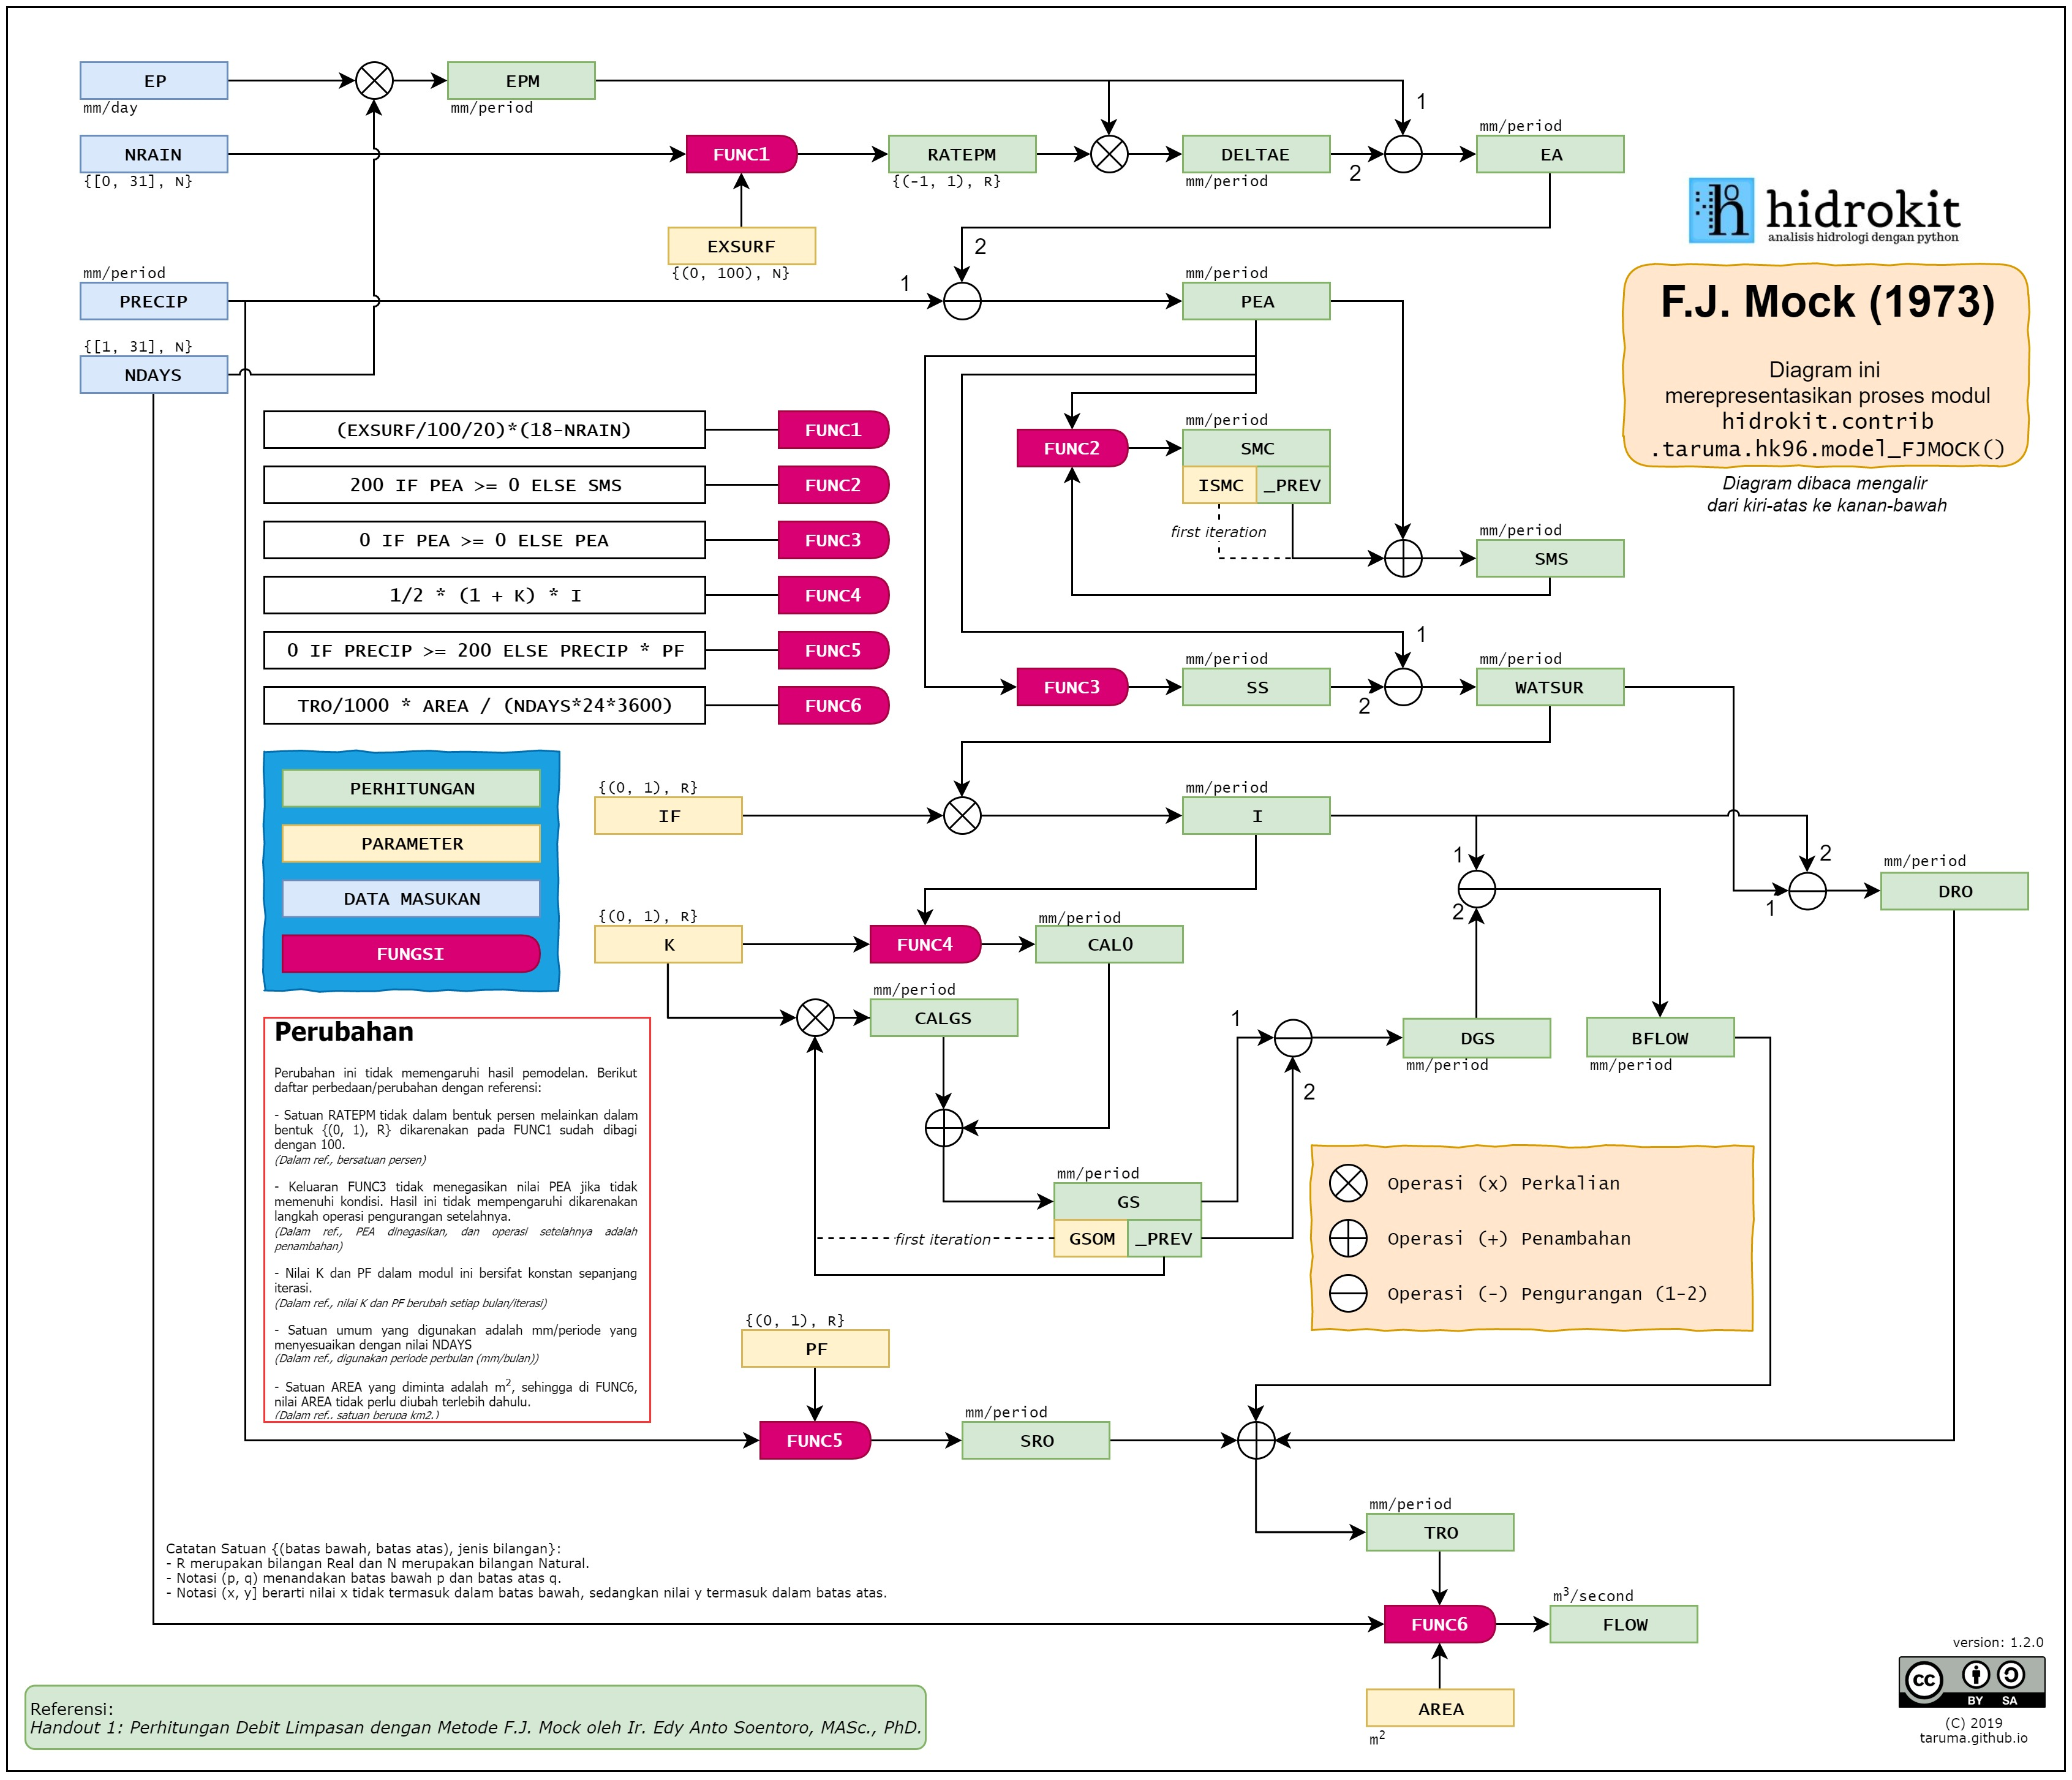
\includegraphics{FJMOCK_hidrokit_1_2_0_300.jpg}
\caption{DIAGRAM FJMOCK}
\end{figure}

Diagram ini bisa diunduh dengan kualitas terbaik
\href{https://github.com/taruma/taruma.github.io/blob/master/assets/hidrokit_assets/FJMOCK_hidrokit_1_2_0_1000.jpg?raw=true}{disini}.
Diagram ini dibuat oleh \href{https://taruma.github.io}{taruma}
menggunakan \href{https://www.draw.io}{draw.io} dengan lisensi
\href{https://creativecommons.org/licenses/by-sa/4.0/}{CC-BY-SA-4.0}.

    \hypertarget{daftar-peubah-dalam-model_fjmock}{%
\subsection{\texorpdfstring{Daftar peubah dalam
\texttt{model\_FJMOCK}}{Daftar peubah dalam model\_FJMOCK}}\label{daftar-peubah-dalam-model_fjmock}}

Berikut daftar peubah yang digunakan dalam \texttt{model\_FJMOCK}:

\begin{longtable}[]{@{}lllc@{}}
\toprule
\begin{minipage}[b]{0.22\columnwidth}\raggedright
Jenis\strut
\end{minipage} & \begin{minipage}[b]{0.22\columnwidth}\raggedright
Peubah\strut
\end{minipage} & \begin{minipage}[b]{0.22\columnwidth}\raggedright
Keterangan\strut
\end{minipage} & \begin{minipage}[b]{0.22\columnwidth}\centering
Satuan\strut
\end{minipage}\tabularnewline
\midrule
\endhead
\begin{minipage}[t]{0.22\columnwidth}\raggedright
\textbf{DATA MASUKAN}\strut
\end{minipage} & \begin{minipage}[t]{0.22\columnwidth}\raggedright
PRECIP\strut
\end{minipage} & \begin{minipage}[t]{0.22\columnwidth}\raggedright
Curah Hujan / Presipitasi\strut
\end{minipage} & \begin{minipage}[t]{0.22\columnwidth}\centering
\(\frac{mm}{period}\)\strut
\end{minipage}\tabularnewline
\begin{minipage}[t]{0.22\columnwidth}\raggedright
.\strut
\end{minipage} & \begin{minipage}[t]{0.22\columnwidth}\raggedright
EP\strut
\end{minipage} & \begin{minipage}[t]{0.22\columnwidth}\raggedright
Evapotranspirasi\strut
\end{minipage} & \begin{minipage}[t]{0.22\columnwidth}\centering
\(^{mm}/_{day}\)\strut
\end{minipage}\tabularnewline
\begin{minipage}[t]{0.22\columnwidth}\raggedright
.\strut
\end{minipage} & \begin{minipage}[t]{0.22\columnwidth}\raggedright
NRAIN\strut
\end{minipage} & \begin{minipage}[t]{0.22\columnwidth}\raggedright
Jumlah hari hujan dalam periode\strut
\end{minipage} & \begin{minipage}[t]{0.22\columnwidth}\centering
\(\{\left[0, 31\right] \in\mathbb{N}\}\)\strut
\end{minipage}\tabularnewline
\begin{minipage}[t]{0.22\columnwidth}\raggedright
.\strut
\end{minipage} & \begin{minipage}[t]{0.22\columnwidth}\raggedright
NDAYS\strut
\end{minipage} & \begin{minipage}[t]{0.22\columnwidth}\raggedright
Jumlah hari dalam periode\strut
\end{minipage} & \begin{minipage}[t]{0.22\columnwidth}\centering
\(\{\left[1, 31\right] \in\mathbb{N}\}\)\strut
\end{minipage}\tabularnewline
\begin{minipage}[t]{0.22\columnwidth}\raggedright
\textbf{PARAMETER}\strut
\end{minipage} & \begin{minipage}[t]{0.22\columnwidth}\raggedright
EXSURF\strut
\end{minipage} & \begin{minipage}[t]{0.22\columnwidth}\raggedright
\emph{Exposed Surface}\strut
\end{minipage} & \begin{minipage}[t]{0.22\columnwidth}\centering
\(\%, \{\left[0, 50\right] \in\mathbb{N}\}\)\strut
\end{minipage}\tabularnewline
\begin{minipage}[t]{0.22\columnwidth}\raggedright
.\strut
\end{minipage} & \begin{minipage}[t]{0.22\columnwidth}\raggedright
IF\strut
\end{minipage} & \begin{minipage}[t]{0.22\columnwidth}\raggedright
\emph{Infiltration Coefficient}\strut
\end{minipage} & \begin{minipage}[t]{0.22\columnwidth}\centering
\(\{\left(0, 1\right) \in\mathbb{R}\}\)\strut
\end{minipage}\tabularnewline
\begin{minipage}[t]{0.22\columnwidth}\raggedright
.\strut
\end{minipage} & \begin{minipage}[t]{0.22\columnwidth}\raggedright
K\strut
\end{minipage} & \begin{minipage}[t]{0.22\columnwidth}\raggedright
\emph{Monthly Flow Recession Constant}\strut
\end{minipage} & \begin{minipage}[t]{0.22\columnwidth}\centering
\(\{\left(0, 1\right) \in\mathbb{R}\}\)\strut
\end{minipage}\tabularnewline
\begin{minipage}[t]{0.22\columnwidth}\raggedright
.\strut
\end{minipage} & \begin{minipage}[t]{0.22\columnwidth}\raggedright
PF\strut
\end{minipage} & \begin{minipage}[t]{0.22\columnwidth}\raggedright
\emph{Percentage Factor}\strut
\end{minipage} & \begin{minipage}[t]{0.22\columnwidth}\centering
\(\{\left(0, 1\right) \in\mathbb{R}\}\)\strut
\end{minipage}\tabularnewline
\begin{minipage}[t]{0.22\columnwidth}\raggedright
.\strut
\end{minipage} & \begin{minipage}[t]{0.22\columnwidth}\raggedright
ISMC\strut
\end{minipage} & \begin{minipage}[t]{0.22\columnwidth}\raggedright
\emph{Initial Soil Moisture Capacity}\strut
\end{minipage} & \begin{minipage}[t]{0.22\columnwidth}\centering
\(\frac{mm}{period}\)\strut
\end{minipage}\tabularnewline
\begin{minipage}[t]{0.22\columnwidth}\raggedright
.\strut
\end{minipage} & \begin{minipage}[t]{0.22\columnwidth}\raggedright
GSOM\strut
\end{minipage} & \begin{minipage}[t]{0.22\columnwidth}\raggedright
\emph{Initial Groundwater Storage}\strut
\end{minipage} & \begin{minipage}[t]{0.22\columnwidth}\centering
\(\frac{mm}{period}\)\strut
\end{minipage}\tabularnewline
\begin{minipage}[t]{0.22\columnwidth}\raggedright
.\strut
\end{minipage} & \begin{minipage}[t]{0.22\columnwidth}\raggedright
AREA\strut
\end{minipage} & \begin{minipage}[t]{0.22\columnwidth}\raggedright
\emph{Catchment Area}\strut
\end{minipage} & \begin{minipage}[t]{0.22\columnwidth}\centering
\(m^2\)\strut
\end{minipage}\tabularnewline
\begin{minipage}[t]{0.22\columnwidth}\raggedright
\textbf{PERHITUNGAN}\strut
\end{minipage} & \begin{minipage}[t]{0.22\columnwidth}\raggedright
EPM\strut
\end{minipage} & \begin{minipage}[t]{0.22\columnwidth}\raggedright
Evapotranspirasi per periode\strut
\end{minipage} & \begin{minipage}[t]{0.22\columnwidth}\centering
\(\frac{mm}{period}\)\strut
\end{minipage}\tabularnewline
\begin{minipage}[t]{0.22\columnwidth}\raggedright
.\strut
\end{minipage} & \begin{minipage}[t]{0.22\columnwidth}\raggedright
RATEPM*\strut
\end{minipage} & \begin{minipage}[t]{0.22\columnwidth}\raggedright
Kalkulasi EXSURF dan NRAIN\strut
\end{minipage} & \begin{minipage}[t]{0.22\columnwidth}\centering
\(\{\left(-1, 1\right) \in\mathbb{R}\}\)\strut
\end{minipage}\tabularnewline
\begin{minipage}[t]{0.22\columnwidth}\raggedright
.\strut
\end{minipage} & \begin{minipage}[t]{0.22\columnwidth}\raggedright
DELTA*\strut
\end{minipage} & \begin{minipage}[t]{0.22\columnwidth}\raggedright
Delta evapotranspirasi\strut
\end{minipage} & \begin{minipage}[t]{0.22\columnwidth}\centering
\(\frac{mm}{period}\)\strut
\end{minipage}\tabularnewline
\begin{minipage}[t]{0.22\columnwidth}\raggedright
.\strut
\end{minipage} & \begin{minipage}[t]{0.22\columnwidth}\raggedright
EA\strut
\end{minipage} & \begin{minipage}[t]{0.22\columnwidth}\raggedright
\emph{Evapotranspirasi Actual}\strut
\end{minipage} & \begin{minipage}[t]{0.22\columnwidth}\centering
\(\frac{mm}{period}\)\strut
\end{minipage}\tabularnewline
\begin{minipage}[t]{0.22\columnwidth}\raggedright
.\strut
\end{minipage} & \begin{minipage}[t]{0.22\columnwidth}\raggedright
PEA*\strut
\end{minipage} & \begin{minipage}[t]{0.22\columnwidth}\raggedright
Kalkulasi P dan EA\strut
\end{minipage} & \begin{minipage}[t]{0.22\columnwidth}\centering
\(\frac{mm}{period}\)\strut
\end{minipage}\tabularnewline
\begin{minipage}[t]{0.22\columnwidth}\raggedright
.\strut
\end{minipage} & \begin{minipage}[t]{0.22\columnwidth}\raggedright
SMS\strut
\end{minipage} & \begin{minipage}[t]{0.22\columnwidth}\raggedright
\emph{Soil Moisture Storage}\strut
\end{minipage} & \begin{minipage}[t]{0.22\columnwidth}\centering
\(\frac{mm}{period}\)\strut
\end{minipage}\tabularnewline
\begin{minipage}[t]{0.22\columnwidth}\raggedright
.\strut
\end{minipage} & \begin{minipage}[t]{0.22\columnwidth}\raggedright
SMC\strut
\end{minipage} & \begin{minipage}[t]{0.22\columnwidth}\raggedright
\emph{Soil Moisture Capacity}\strut
\end{minipage} & \begin{minipage}[t]{0.22\columnwidth}\centering
\(\frac{mm}{period}\)\strut
\end{minipage}\tabularnewline
\begin{minipage}[t]{0.22\columnwidth}\raggedright
.\strut
\end{minipage} & \begin{minipage}[t]{0.22\columnwidth}\raggedright
SS\strut
\end{minipage} & \begin{minipage}[t]{0.22\columnwidth}\raggedright
\emph{Soil Storage}\strut
\end{minipage} & \begin{minipage}[t]{0.22\columnwidth}\centering
\(\frac{mm}{period}\)\strut
\end{minipage}\tabularnewline
\begin{minipage}[t]{0.22\columnwidth}\raggedright
.\strut
\end{minipage} & \begin{minipage}[t]{0.22\columnwidth}\raggedright
I\strut
\end{minipage} & \begin{minipage}[t]{0.22\columnwidth}\raggedright
\emph{Infiltration}\strut
\end{minipage} & \begin{minipage}[t]{0.22\columnwidth}\centering
\(\frac{mm}{period}\)\strut
\end{minipage}\tabularnewline
\begin{minipage}[t]{0.22\columnwidth}\raggedright
.\strut
\end{minipage} & \begin{minipage}[t]{0.22\columnwidth}\raggedright
CAL0*\strut
\end{minipage} & \begin{minipage}[t]{0.22\columnwidth}\raggedright
Kalkulasi K dan I\strut
\end{minipage} & \begin{minipage}[t]{0.22\columnwidth}\centering
\(\frac{mm}{period}\)\strut
\end{minipage}\tabularnewline
\begin{minipage}[t]{0.22\columnwidth}\raggedright
.\strut
\end{minipage} & \begin{minipage}[t]{0.22\columnwidth}\raggedright
CALGS*\strut
\end{minipage} & \begin{minipage}[t]{0.22\columnwidth}\raggedright
Kalkulasi K dan GS\_PREV/GSOM\strut
\end{minipage} & \begin{minipage}[t]{0.22\columnwidth}\centering
\(\frac{mm}{period}\)\strut
\end{minipage}\tabularnewline
\begin{minipage}[t]{0.22\columnwidth}\raggedright
.\strut
\end{minipage} & \begin{minipage}[t]{0.22\columnwidth}\raggedright
GS\strut
\end{minipage} & \begin{minipage}[t]{0.22\columnwidth}\raggedright
\emph{Groundwater Storage}\strut
\end{minipage} & \begin{minipage}[t]{0.22\columnwidth}\centering
\(\frac{mm}{period}\)\strut
\end{minipage}\tabularnewline
\begin{minipage}[t]{0.22\columnwidth}\raggedright
.\strut
\end{minipage} & \begin{minipage}[t]{0.22\columnwidth}\raggedright
DGS\strut
\end{minipage} & \begin{minipage}[t]{0.22\columnwidth}\raggedright
\emph{Delta Groundwater Storage}\strut
\end{minipage} & \begin{minipage}[t]{0.22\columnwidth}\centering
\(\frac{mm}{period}\)\strut
\end{minipage}\tabularnewline
\begin{minipage}[t]{0.22\columnwidth}\raggedright
.\strut
\end{minipage} & \begin{minipage}[t]{0.22\columnwidth}\raggedright
BFLOW\strut
\end{minipage} & \begin{minipage}[t]{0.22\columnwidth}\raggedright
\emph{Base Flow}\strut
\end{minipage} & \begin{minipage}[t]{0.22\columnwidth}\centering
\(\frac{mm}{period}\)\strut
\end{minipage}\tabularnewline
\begin{minipage}[t]{0.22\columnwidth}\raggedright
.\strut
\end{minipage} & \begin{minipage}[t]{0.22\columnwidth}\raggedright
DRO\strut
\end{minipage} & \begin{minipage}[t]{0.22\columnwidth}\raggedright
\emph{Direct Runoff}\strut
\end{minipage} & \begin{minipage}[t]{0.22\columnwidth}\centering
\(\frac{mm}{period}\)\strut
\end{minipage}\tabularnewline
\begin{minipage}[t]{0.22\columnwidth}\raggedright
.\strut
\end{minipage} & \begin{minipage}[t]{0.22\columnwidth}\raggedright
SRO\strut
\end{minipage} & \begin{minipage}[t]{0.22\columnwidth}\raggedright
\emph{Storm Runoff}\strut
\end{minipage} & \begin{minipage}[t]{0.22\columnwidth}\centering
\(\frac{mm}{period}\)\strut
\end{minipage}\tabularnewline
\begin{minipage}[t]{0.22\columnwidth}\raggedright
.\strut
\end{minipage} & \begin{minipage}[t]{0.22\columnwidth}\raggedright
TRO\strut
\end{minipage} & \begin{minipage}[t]{0.22\columnwidth}\raggedright
\emph{Total Runoff}\strut
\end{minipage} & \begin{minipage}[t]{0.22\columnwidth}\centering
\(\frac{mm}{period}\)\strut
\end{minipage}\tabularnewline
\begin{minipage}[t]{0.22\columnwidth}\raggedright
.\strut
\end{minipage} & \begin{minipage}[t]{0.22\columnwidth}\raggedright
FLOW\strut
\end{minipage} & \begin{minipage}[t]{0.22\columnwidth}\raggedright
\emph{Stream Flow}\strut
\end{minipage} & \begin{minipage}[t]{0.22\columnwidth}\centering
\(\frac{m^{3}}{second}\)\strut
\end{minipage}\tabularnewline
\bottomrule
\end{longtable}

Catatan:

\begin{itemize}
\tightlist
\item
  \_PREV: Nilai pada iterasi sebelumnya \((j-1)\).
\item
  *: Nama peubah ini dibuat khusus untuk fungsi \texttt{model\_FJMOCK}
  (tidak mengikuti/ada pada referensi).
\end{itemize}

    \hypertarget{fungsi}{%
\section{FUNGSI}\label{fungsi}}

    \hypertarget{fungsi-model_fjmock}{%
\subsection{\texorpdfstring{Fungsi
\texttt{model\_FJMOCK}}{Fungsi model\_FJMOCK}}\label{fungsi-model_fjmock}}

Fungsi \texttt{model\_FJMOCK} membangkitkan nilai debit menggunakan
model yang dikembangkan oleh Dr.~F. J. Mock (Mock 1973). Untuk
mengetahui masing-masing batasan model ini, harap melihat pada referensi
topik terkait. Dalam \emph{notebook} ini hanya fokus pada penggunaan
fungsi.

Fungsi memiliki 12 argumen yang harus diisi, dan 2 argumen opsional.
Dibagi menjadi 3 bagian argumen yaitu:

\begin{itemize}
\tightlist
\item
  Argumen untuk dataset:

  \begin{itemize}
  \tightlist
  \item
    \texttt{df}: dataset dalam objek \texttt{pandas.DataFrame}.
  \item
    \texttt{precip\_col}: nama kolom curah hujan (presipitasi).
  \item
    \texttt{ep\_col}: nama kolom evapotranspirasi.
  \item
    \texttt{nrain\_col}: nama kolom jumlah hari hujan dalam periode.
  \item
    \texttt{ndays\_col}: nama kolom jumlah hari dalam periode.
  \end{itemize}
\item
  Argumen untuk parameter model:

  \begin{itemize}
  \tightlist
  \item
    \texttt{EXSURF}: \emph{Exposed Surface}.
  \item
    \texttt{IF}: \emph{Infiltration Coefficient}.
  \item
    \texttt{K}: \emph{Monthly Flow Recession Constant}.
  \item
    \texttt{PF}: \emph{Percentage Factor}.
  \item
    \texttt{ISMC}: \emph{Initial Soil Moisture Capacity}.
  \item
    \texttt{GSOM}: \emph{Initial Groundwater Storage}.
  \item
    \texttt{AREA}: \emph{Catchment Area}.
  \end{itemize}
\item
  Argumen opsional untuk fungsi:

  \begin{itemize}
  \tightlist
  \item
    \texttt{as\_df}: \texttt{True} (\emph{default}), keluaran berupa
    \texttt{pandas.DataFrame}. Keluaran berupa \texttt{numpy.ndarray}
    jika \texttt{False}.
  \item
    \texttt{report}: \texttt{\textquotesingle{}flow\textquotesingle{}}
    (\emph{default}), terdapat beberapa nilai yang diterima oleh argumen
    \texttt{report}:

    \begin{itemize}
    \tightlist
    \item
      \texttt{full}: keluaran akan menyertakan seluruh peubah yang
      dihitung dalam model.
    \item
      \texttt{partial}: keluaran hanya menyertakan kolom
      \texttt{PRECIP}, \texttt{NRAIN}, \texttt{NDAYS}, \texttt{EP},
      \texttt{EA}, \texttt{SMS}, \texttt{SS}, \texttt{GS}, \texttt{TRO},
      \texttt{FLOW}.
    \item
      \texttt{tro}: keluaran hanya menyertakan kolom \texttt{TRO}.
    \item
      \texttt{flow}: keluaran hanya menyertakan kolom \texttt{FLOW}.
    \end{itemize}
  \end{itemize}
\end{itemize}

    \hypertarget{as_dftrue-reportflow-default}{%
\subsubsection{\texorpdfstring{\texttt{as\_df=True},
\texttt{report=\textquotesingle{}flow\textquotesingle{}}
(\emph{default})}{as\_df=True, report='flow' (default)}}\label{as_dftrue-reportflow-default}}

Keluaran berupa \texttt{pandas.DataFrame}.

    \begin{tcolorbox}[breakable, size=fbox, boxrule=1pt, pad at break*=1mm,colback=cellbackground, colframe=cellborder]
\prompt{In}{incolor}{0}{\boxspacing}
\begin{Verbatim}[commandchars=\\\{\}]
\PY{n}{model\PYZus{}FJMOCK}\PY{p}{(}\PY{n}{dataset}\PY{p}{,}
             \PY{n}{precip\PYZus{}col}\PY{o}{=}\PY{l+s+s1}{\PYZsq{}}\PY{l+s+s1}{PRECIP}\PY{l+s+s1}{\PYZsq{}}\PY{p}{,} \PY{n}{ep\PYZus{}col}\PY{o}{=}\PY{l+s+s1}{\PYZsq{}}\PY{l+s+s1}{PET}\PY{l+s+s1}{\PYZsq{}}\PY{p}{,} \PY{n}{nrain\PYZus{}col}\PY{o}{=}\PY{l+s+s1}{\PYZsq{}}\PY{l+s+s1}{NRAIN}\PY{l+s+s1}{\PYZsq{}}\PY{p}{,} 
             \PY{n}{ndays\PYZus{}col}\PY{o}{=}\PY{l+s+s1}{\PYZsq{}}\PY{l+s+s1}{NDAYS}\PY{l+s+s1}{\PYZsq{}}\PY{p}{,}
             \PY{n}{EXSURF}\PY{o}{=}\PY{l+m+mi}{40}\PY{p}{,} \PY{n}{IF}\PY{o}{=}\PY{l+m+mf}{0.7}\PY{p}{,} \PY{n}{K}\PY{o}{=}\PY{l+m+mf}{0.6}\PY{p}{,} \PY{n}{PF}\PY{o}{=}\PY{l+m+mf}{0.2}\PY{p}{,} \PY{n}{ISMC}\PY{o}{=}\PY{l+m+mi}{200}\PY{p}{,} \PY{n}{GSOM}\PY{o}{=}\PY{l+m+mf}{215.8}\PY{p}{,} 
             \PY{n}{AREA}\PY{o}{=}\PY{l+m+mf}{291.83e6}\PY{p}{)}\PY{o}{.}\PY{n}{head}\PY{p}{(}\PY{p}{)}
\end{Verbatim}
\end{tcolorbox}

            \begin{tcolorbox}[breakable, size=fbox, boxrule=.5pt, pad at break*=1mm, opacityfill=0]
\prompt{Out}{outcolor}{0}{\boxspacing}
\begin{Verbatim}[commandchars=\\\{\}]
                 FLOW
2005-01-01  11.038314
2005-02-01   7.524411
2005-03-01   5.427550
2005-04-01   4.200750
2005-05-01   1.476165
\end{Verbatim}
\end{tcolorbox}
        
    sebagian argumen bisa disimpan dalam bentuk \emph{dictionary}.

    \begin{tcolorbox}[breakable, size=fbox, boxrule=1pt, pad at break*=1mm,colback=cellbackground, colframe=cellborder]
\prompt{In}{incolor}{0}{\boxspacing}
\begin{Verbatim}[commandchars=\\\{\}]
\PY{n}{parameter} \PY{o}{=} \PY{p}{\PYZob{}}
    \PY{l+s+s1}{\PYZsq{}}\PY{l+s+s1}{EXSURF}\PY{l+s+s1}{\PYZsq{}}\PY{p}{:} \PY{l+m+mi}{40}\PY{p}{,}
    \PY{l+s+s1}{\PYZsq{}}\PY{l+s+s1}{IF}\PY{l+s+s1}{\PYZsq{}}\PY{p}{:} \PY{l+m+mf}{0.7}\PY{p}{,}
    \PY{l+s+s1}{\PYZsq{}}\PY{l+s+s1}{K}\PY{l+s+s1}{\PYZsq{}}\PY{p}{:} \PY{l+m+mf}{0.6}\PY{p}{,}
    \PY{l+s+s1}{\PYZsq{}}\PY{l+s+s1}{PF}\PY{l+s+s1}{\PYZsq{}}\PY{p}{:} \PY{l+m+mf}{0.2}\PY{p}{,}
    \PY{l+s+s1}{\PYZsq{}}\PY{l+s+s1}{ISMC}\PY{l+s+s1}{\PYZsq{}}\PY{p}{:} \PY{l+m+mi}{200}\PY{p}{,}
    \PY{l+s+s1}{\PYZsq{}}\PY{l+s+s1}{GSOM}\PY{l+s+s1}{\PYZsq{}}\PY{p}{:} \PY{l+m+mf}{215.8}\PY{p}{,}
    \PY{l+s+s1}{\PYZsq{}}\PY{l+s+s1}{AREA}\PY{l+s+s1}{\PYZsq{}}\PY{p}{:} \PY{l+m+mf}{291.83e6}
\PY{p}{\PYZcb{}}

\PY{n}{dataset\PYZus{}params} \PY{o}{=} \PY{p}{\PYZob{}}
    \PY{l+s+s1}{\PYZsq{}}\PY{l+s+s1}{precip\PYZus{}col}\PY{l+s+s1}{\PYZsq{}}\PY{p}{:} \PY{l+s+s1}{\PYZsq{}}\PY{l+s+s1}{PRECIP}\PY{l+s+s1}{\PYZsq{}}\PY{p}{,}
    \PY{l+s+s1}{\PYZsq{}}\PY{l+s+s1}{ep\PYZus{}col}\PY{l+s+s1}{\PYZsq{}}\PY{p}{:} \PY{l+s+s1}{\PYZsq{}}\PY{l+s+s1}{PET}\PY{l+s+s1}{\PYZsq{}}\PY{p}{,}
    \PY{l+s+s1}{\PYZsq{}}\PY{l+s+s1}{nrain\PYZus{}col}\PY{l+s+s1}{\PYZsq{}}\PY{p}{:} \PY{l+s+s1}{\PYZsq{}}\PY{l+s+s1}{NRAIN}\PY{l+s+s1}{\PYZsq{}}\PY{p}{,}
    \PY{l+s+s1}{\PYZsq{}}\PY{l+s+s1}{ndays\PYZus{}col}\PY{l+s+s1}{\PYZsq{}}\PY{p}{:} \PY{l+s+s1}{\PYZsq{}}\PY{l+s+s1}{NDAYS}\PY{l+s+s1}{\PYZsq{}}
\PY{p}{\PYZcb{}}

\PY{n}{model\PYZus{}FJMOCK}\PY{p}{(}\PY{n}{dataset}\PY{p}{,}
             \PY{o}{*}\PY{o}{*}\PY{n}{dataset\PYZus{}params}\PY{p}{,}
             \PY{o}{*}\PY{o}{*}\PY{n}{parameter}\PY{p}{)}\PY{o}{.}\PY{n}{head}\PY{p}{(}\PY{p}{)}
\end{Verbatim}
\end{tcolorbox}

            \begin{tcolorbox}[breakable, size=fbox, boxrule=.5pt, pad at break*=1mm, opacityfill=0]
\prompt{Out}{outcolor}{0}{\boxspacing}
\begin{Verbatim}[commandchars=\\\{\}]
                 FLOW
2005-01-01  11.038314
2005-02-01   7.524411
2005-03-01   5.427550
2005-04-01   4.200750
2005-05-01   1.476165
\end{Verbatim}
\end{tcolorbox}
        
    \hypertarget{as_dffalse}{%
\subsubsection{\texorpdfstring{\texttt{as\_df=False}}{as\_df=False}}\label{as_dffalse}}

Keluaran berupa \texttt{numpy.ndarray}

    \begin{tcolorbox}[breakable, size=fbox, boxrule=1pt, pad at break*=1mm,colback=cellbackground, colframe=cellborder]
\prompt{In}{incolor}{0}{\boxspacing}
\begin{Verbatim}[commandchars=\\\{\}]
\PY{n}{model\PYZus{}FJMOCK}\PY{p}{(}\PY{n}{dataset}\PY{p}{,} \PY{o}{*}\PY{o}{*}\PY{n}{dataset\PYZus{}params}\PY{p}{,} \PY{o}{*}\PY{o}{*}\PY{n}{parameter}\PY{p}{,}
             \PY{n}{as\PYZus{}df}\PY{o}{=}\PY{k+kc}{False}\PY{p}{)}
\end{Verbatim}
\end{tcolorbox}

            \begin{tcolorbox}[breakable, size=fbox, boxrule=.5pt, pad at break*=1mm, opacityfill=0]
\prompt{Out}{outcolor}{0}{\boxspacing}
\begin{Verbatim}[commandchars=\\\{\}]
array([11.03831372,  7.52441118,  5.42754989,  4.20074969,  1.4761652 ,
        1.33453689,  1.02392803,  0.99639442,  0.31482649,  0.96645418,
        0.63746247,  4.39633798,  6.71094135,  7.20975475,  3.60403751,
        3.40811612,  1.89545724,  0.57464413,  0.26752973,  0.16051784,
        0.09952106,  0.32607131,  1.19601734,  1.97546623,  0.78477441,
        1.40605689,  3.96837248,  2.74163501,  0.82829662,  0.33280309,
        0.15150419,  0.17996924,  0.17930671,  0.60706392,  1.42338245,
        4.51935998,  5.48703509,  7.86158518,  6.66854605,  4.61270398,
        1.80639153,  1.05273253,  0.55782402,  0.60313774,  0.86819483,
        1.56157215,  2.58970373,  2.53405371,  2.42960495,  3.33457675,
        2.18728535,  1.7071079 ,  1.36990622,  1.67615626,  0.11338267,
        0.03593304,  0.65775625,  0.6697543 ,  0.86505161,  2.17619576,
        1.70680932,  0.91144292,  3.44637769,  3.19805379,  5.71876288,
        2.28340161,  1.16355342,  1.21896099,  1.97557412,  3.34579081,
        1.92074562,  4.33700229,  2.73683673,  2.9936993 ,  2.29876246,
        1.83275104,  1.42160582,  0.46468883,  0.16007029,  0.0408782 ,
        0.68439159,  1.24573648,  6.0382106 ,  3.82709625,  6.98086936,
        4.04282714,  2.94190223,  2.25193748,  1.00004163,  0.75235851,
        0.1507685 ,  0.0904611 ,  0.08961692,  0.83990998,  4.64925624,
        3.68580346,  3.87585627,  2.26932747,  1.97068683,  1.56419699,
        1.81200324,  3.66691915,  1.99050686,  1.0237562 ,  0.97876111,
        1.80306937,  4.62827508,  7.05110499,  9.87122757,  5.9298505 ,
        2.34081328,  3.21261903,  1.91956054,  3.96141509,  2.7031486 ,
        1.36212155,  1.00132982,  4.06325897,  1.16137442,  4.18293059,
        8.3877247 , 10.95612413,  9.73624701,  8.70589257,  3.78714981,
        3.53442349,  1.40204959,  0.6562682 ,  0.63601507,  0.8963778 ,
        5.17469187,  3.04163336])
\end{Verbatim}
\end{tcolorbox}
        
    \hypertarget{report}{%
\subsubsection{\texorpdfstring{\texttt{report}}{report}}\label{report}}

    \hypertarget{reportfull}{%
\paragraph{\texorpdfstring{\texttt{report=\textquotesingle{}full\textquotesingle{}}}{report='full'}}\label{reportfull}}

    \begin{tcolorbox}[breakable, size=fbox, boxrule=1pt, pad at break*=1mm,colback=cellbackground, colframe=cellborder]
\prompt{In}{incolor}{0}{\boxspacing}
\begin{Verbatim}[commandchars=\\\{\}]
\PY{n}{model\PYZus{}FJMOCK}\PY{p}{(}\PY{n}{dataset}\PY{p}{,} \PY{o}{*}\PY{o}{*}\PY{n}{dataset\PYZus{}params}\PY{p}{,} \PY{o}{*}\PY{o}{*}\PY{n}{parameter}\PY{p}{,}
             \PY{n}{report}\PY{o}{=}\PY{l+s+s1}{\PYZsq{}}\PY{l+s+s1}{full}\PY{l+s+s1}{\PYZsq{}}\PY{p}{)}
\end{Verbatim}
\end{tcolorbox}

            \begin{tcolorbox}[breakable, size=fbox, boxrule=.5pt, pad at break*=1mm, opacityfill=0]
\prompt{Out}{outcolor}{0}{\boxspacing}
\begin{Verbatim}[commandchars=\\\{\}]
                PRECIP  NRAIN  NDAYS  {\ldots}        SRO         TRO       FLOW
2005-01-01   74.945240   19.0   31.0  {\ldots}  14.989048  101.309048  11.038314
2005-02-01   52.917729   12.0   28.0  {\ldots}  10.583546   62.375546   7.524411
2005-03-01   93.692801   17.0   31.0  {\ldots}  18.738560   49.813760   5.427550
2005-04-01   93.327242   19.0   30.0  {\ldots}  18.665448   37.310568   4.200750
2005-05-01   11.805463    7.0   31.0  {\ldots}   2.361093   13.548165   1.476165
{\ldots}                {\ldots}    {\ldots}    {\ldots}  {\ldots}        {\ldots}         {\ldots}        {\ldots}
2015-08-01    0.000000    0.0   31.0  {\ldots}   0.000000    6.023194   0.656268
2015-09-01   10.175476    3.0   30.0  {\ldots}   2.035095    5.649012   0.636015
2015-10-01   30.292786   12.0   31.0  {\ldots}   6.058557    8.226907   0.896378
2015-11-01  161.871088   25.0   30.0  {\ldots}  32.374218   45.961009   5.174692
2015-12-01  104.403805   25.0   31.0  {\ldots}  20.880761   27.915947   3.041633

[132 rows x 23 columns]
\end{Verbatim}
\end{tcolorbox}
        
    \hypertarget{reportpartial}{%
\paragraph{\texorpdfstring{\texttt{report=\textquotesingle{}partial\textquotesingle{}}}{report='partial'}}\label{reportpartial}}

    \begin{tcolorbox}[breakable, size=fbox, boxrule=1pt, pad at break*=1mm,colback=cellbackground, colframe=cellborder]
\prompt{In}{incolor}{0}{\boxspacing}
\begin{Verbatim}[commandchars=\\\{\}]
\PY{n}{model\PYZus{}FJMOCK}\PY{p}{(}\PY{n}{dataset}\PY{p}{,} \PY{o}{*}\PY{o}{*}\PY{n}{dataset\PYZus{}params}\PY{p}{,} \PY{o}{*}\PY{o}{*}\PY{n}{parameter}\PY{p}{,}
             \PY{n}{report}\PY{o}{=}\PY{l+s+s1}{\PYZsq{}}\PY{l+s+s1}{partial}\PY{l+s+s1}{\PYZsq{}}\PY{p}{)}
\end{Verbatim}
\end{tcolorbox}

            \begin{tcolorbox}[breakable, size=fbox, boxrule=.5pt, pad at break*=1mm, opacityfill=0]
\prompt{Out}{outcolor}{0}{\boxspacing}
\begin{Verbatim}[commandchars=\\\{\}]
                PRECIP  NRAIN  NDAYS  {\ldots}          GS         TRO       FLOW
2005-01-01   74.945240   19.0   31.0  {\ldots}  129.480000  101.309048  11.038314
2005-02-01   52.917729   12.0   28.0  {\ldots}   77.688000   62.375546   7.524411
2005-03-01   93.692801   17.0   31.0  {\ldots}   46.612800   49.813760   5.427550
2005-04-01   93.327242   19.0   30.0  {\ldots}   27.967680   37.310568   4.200750
2005-05-01   11.805463    7.0   31.0  {\ldots}   16.780608   13.548165   1.476165
{\ldots}                {\ldots}    {\ldots}    {\ldots}  {\ldots}         {\ldots}         {\ldots}        {\ldots}
2015-08-01    0.000000    0.0   31.0  {\ldots}    9.034791    6.023194   0.656268
2015-09-01   10.175476    3.0   30.0  {\ldots}    5.420875    5.649012   0.636015
2015-10-01   30.292786   12.0   31.0  {\ldots}    3.252525    8.226907   0.896378
2015-11-01  161.871088   25.0   30.0  {\ldots}   17.587965   45.961009   5.174692
2015-12-01  104.403805   25.0   31.0  {\ldots}   10.552779   27.915947   3.041633

[132 rows x 10 columns]
\end{Verbatim}
\end{tcolorbox}
        
    \hypertarget{reporttro}{%
\paragraph{\texorpdfstring{\texttt{report=\textquotesingle{}tro\textquotesingle{}}}{report='tro'}}\label{reporttro}}

    \begin{tcolorbox}[breakable, size=fbox, boxrule=1pt, pad at break*=1mm,colback=cellbackground, colframe=cellborder]
\prompt{In}{incolor}{0}{\boxspacing}
\begin{Verbatim}[commandchars=\\\{\}]
\PY{n}{model\PYZus{}FJMOCK}\PY{p}{(}\PY{n}{dataset}\PY{p}{,} \PY{o}{*}\PY{o}{*}\PY{n}{dataset\PYZus{}params}\PY{p}{,} \PY{o}{*}\PY{o}{*}\PY{n}{parameter}\PY{p}{,}
             \PY{n}{report}\PY{o}{=}\PY{l+s+s1}{\PYZsq{}}\PY{l+s+s1}{tro}\PY{l+s+s1}{\PYZsq{}}\PY{p}{)}
\end{Verbatim}
\end{tcolorbox}

            \begin{tcolorbox}[breakable, size=fbox, boxrule=.5pt, pad at break*=1mm, opacityfill=0]
\prompt{Out}{outcolor}{0}{\boxspacing}
\begin{Verbatim}[commandchars=\\\{\}]
                   TRO
2005-01-01  101.309048
2005-02-01   62.375546
2005-03-01   49.813760
2005-04-01   37.310568
2005-05-01   13.548165
{\ldots}                {\ldots}
2015-08-01    6.023194
2015-09-01    5.649012
2015-10-01    8.226907
2015-11-01   45.961009
2015-12-01   27.915947

[132 rows x 1 columns]
\end{Verbatim}
\end{tcolorbox}
        
    \hypertarget{reportflow-default}{%
\paragraph{\texorpdfstring{\texttt{report=\textquotesingle{}flow\textquotesingle{}}
(\emph{default})}{report='flow' (default)}}\label{reportflow-default}}

    \begin{tcolorbox}[breakable, size=fbox, boxrule=1pt, pad at break*=1mm,colback=cellbackground, colframe=cellborder]
\prompt{In}{incolor}{0}{\boxspacing}
\begin{Verbatim}[commandchars=\\\{\}]
\PY{n}{model\PYZus{}FJMOCK}\PY{p}{(}\PY{n}{dataset}\PY{p}{,} \PY{o}{*}\PY{o}{*}\PY{n}{dataset\PYZus{}params}\PY{p}{,} \PY{o}{*}\PY{o}{*}\PY{n}{parameter}\PY{p}{,}
             \PY{n}{report}\PY{o}{=}\PY{l+s+s1}{\PYZsq{}}\PY{l+s+s1}{flow}\PY{l+s+s1}{\PYZsq{}}\PY{p}{)}
\end{Verbatim}
\end{tcolorbox}

            \begin{tcolorbox}[breakable, size=fbox, boxrule=.5pt, pad at break*=1mm, opacityfill=0]
\prompt{Out}{outcolor}{0}{\boxspacing}
\begin{Verbatim}[commandchars=\\\{\}]
                 FLOW
2005-01-01  11.038314
2005-02-01   7.524411
2005-03-01   5.427550
2005-04-01   4.200750
2005-05-01   1.476165
{\ldots}               {\ldots}
2015-08-01   0.656268
2015-09-01   0.636015
2015-10-01   0.896378
2015-11-01   5.174692
2015-12-01   3.041633

[132 rows x 1 columns]
\end{Verbatim}
\end{tcolorbox}
        
    \hypertarget{changelog}{%
\section{Changelog}\label{changelog}}

\begin{verbatim}
- 20191218 - 1.1.0 - Initial
\end{verbatim}

\hypertarget{copyright-2019-taruma-sakti-megariansyah}{%
\paragraph{\texorpdfstring{Copyright © 2019
\href{https://taruma.github.io}{Taruma Sakti
Megariansyah}}{Copyright © 2019 Taruma Sakti Megariansyah}}\label{copyright-2019-taruma-sakti-megariansyah}}

Source code in this notebook is licensed under a
\href{https://choosealicense.com/licenses/mit/}{MIT License}. Data in
this notebook is licensed under a
\href{https://creativecommons.org/licenses/by/4.0/}{Creative Common
Attribution 4.0 International}.


    % Add a bibliography block to the postdoc
    
    
    
\end{document}
